% 由 tools/md2tex.py 自 2023_数学真题_新高考Ⅱ_含解析.md 生成，勿手改（改源 MD 后重跑）


\begin{gknotice}
\textbf{来源说明}：试题原文取自 deekur/gaokaomath（commit \texttt{34c13a6}，CC BY 4.0）之「2023新高考2」PDF，逐题照图转录。

\textbf{解析归属}：本文档全部解析由本库编写者根据试题独立推导，\textbf{非官方标准答案}。推导过程完整给出以便核验；若与官方发布版本不一致，以官方为准。

\textbf{结构提示}：本卷为 22 题制。2024 年起改为 19 题制，故本卷宜按知识点抽题练习，不宜整套限时模拟。
\end{gknotice}

\par\medskip

\gkpart{一、单选题（每小题 5 分，共 40 分）}

\gksolhead{1}{}

\textbf{题目}　在复平面内，$(1+3\mathrm i)(3-\mathrm i)$ 对应的点位于（　　）

\textbf{解析}

按多项式展开，注意 $\mathrm i^{2}=-1$：
\[(1+3\mathrm i)(3-\mathrm i)=1\times3+1\times(-\mathrm i)+3\mathrm i\times3+3\mathrm i\times(-\mathrm i)\]

\[=3-\mathrm i+9\mathrm i-3\mathrm i^{2}=3+8\mathrm i+3=6+8\mathrm i\]

对应的点为 $(6,8)$，横、纵坐标均为正，位于\textbf{第一象限}。

\gkanswer{答案：A}

\begin{gktip}
\textbf{提速技巧}：只判象限时不必算完整乘积，只要\textbf{实部与虚部的符号}。也可用辐角相加：$1+3\mathrm i$ 的辐角在第一象限（约 $71.6^\circ$），$3-\mathrm i$ 的辐角在第四象限（约 $-18.4^\circ$），和约 $53.2^\circ$，仍在第一象限。
\end{gktip}

\par\medskip

\gksolhead{2}{}

\textbf{题目}　设集合 $A=\{0,-a\}$，$B=\{1,a-2,2a-2\}$，若 $A\subseteq B$，则 $a=$（　　）

\textbf{解析}

\textbf{第一步，用 $0\in A$ 锁定候选值。}

$A\subseteq B$ 要求 $A$ 的每个元素都在 $B$ 中，先看 $0$：因 $1\ne0$，必有
\[a-2=0\quad\text{\text{或}}\quad 2a-2=0\]

即 $a=2$ 或 $a=1$。\textbf{这一步把无穷多种可能压缩成两种}，是本题的关键。

\textbf{第二步，逐一代回检验（必须做，否则会误选）。}

\begin{center}
\begin{tabular}{cccc}
\toprule
候选 & $A$ & $B$ & 结论 \\
\midrule
$a=2$ & $\{0,-2\}$ & $\{1,0,2\}$ & $-2\notin B$， \\
$a=1$ & $\{0,-1\}$ & $\{1,-1,0\}$ & 两元素均在 $B$ 中， \\
\bottomrule
\end{tabular}
\end{center}

$a=1$ 时还需检验集合的\textbf{互异性}：$A=\{0,-1\}$ 两元素不同 ；$B=\{1,-1,0\}$ 三元素互不相同 。故 $a=1$ 合法。

\gkanswer{答案：B}

\begin{gktip}
\textbf{易错点}：只做第一步就选 A（$a=2$）是本题最常见的失分方式。$0\in B$ 是 $A\subseteq B$ 的\textbf{必要条件而非充分条件}，必须把 $-a$ 也验一遍。另外，含参数的集合题\textbf{永远要回代检验互异性}。
\end{gktip}

\par\medskip

\gksolhead{3}{}

\textbf{题目}　某学校为了解学生参加体育运动的情况，用比例分配的分层随机抽样法作抽样调查，拟从初中部和高中部两层共抽取 $60$ 名学生，已知该校初中部和高中部分别有 $400$ 名和 $200$ 名学生，则不同的抽样结果共有（　　）

\textbf{解析}

\textbf{第一步，按比例分配确定各层的抽取人数。}

总体共 $400+200=600$ 人，抽样比
\[k=\frac{60}{600}=\frac1{10}\]

于是
\[\text{\text{初中部抽}}\ 400\times\frac1{10}=40\ \text{\text{人}},\qquad \text{\text{高中部抽}}\ 200\times\frac1{10}=20\ \text{\text{人}}\]

\textbf{第二步，计数。}

初中部的 $40$ 人从 $400$ 人中选：$C_{400}^{40}$ 种；高中部的 $20$ 人从 $200$ 人中选：$C_{200}^{20}$ 种。两层的选择互相独立，由\textbf{分步乘法计数原理}：
\[N=C_{400}^{40}C_{200}^{20}\]

\gkanswer{答案：D}

\begin{gktip}
\textbf{辨析}：选项 C（$C_{400}^{30}C_{200}^{30}$）对应的是「每层各抽 $30$ 人」的\textbf{等额分配}，不是比例分配；选项 B 把两层的人数\textbf{抽反了}（从 $400$ 人里抽 $20$、从 $200$ 人里抽 $40$）。看到「比例分配」四字，第一动作就是算抽样比。
\end{gktip}

\par\medskip

\gksolhead{4}{}

\textbf{题目}　若 $f(x)=(x+a)\ln\dfrac{2x-1}{2x+1}$ 为偶函数，则 $a=$（　　）

\textbf{解析}

\textbf{第一步，确认定义域关于原点对称（偶函数的前提）。}

需 $\dfrac{2x-1}{2x+1}>0$，即 $x>\dfrac12$ 或 $x<-\dfrac12$。定义域
\[D=\left(-\infty,-\frac12\right)\cup\left(\frac12,+\infty\right)\]
关于原点对称 

\textbf{第二步，识别对数因子是奇函数。}

记 $g(x)=\ln\dfrac{2x-1}{2x+1}$，则
\[g(-x)=\ln\frac{-2x-1}{-2x+1}=\ln\frac{2x+1}{2x-1}=\ln\left(\frac{2x-1}{2x+1}\right)^{-1}=-g(x)\]

故 $g$ 是\textbf{奇函数}。

\textbf{第三步，由「偶 $=$ 奇 $\times$ 奇」定出 $a$。}

\[f(-x)=(-x+a)g(-x)=(-x+a)\left(-g(x)\right)=(x-a)g(x)\]

$f$ 为偶函数即 $f(-x)=f(x)$ 对一切 $x\in D$ 成立：
\[(x-a)g(x)=(x+a)g(x)\ \Longrightarrow\ 2a\,g(x)=0\]

而 $g(x)=0$ 需要 $\dfrac{2x-1}{2x+1}=1$，即 $-1=1$，\textbf{不可能}，故 $g(x)\ne0$ 恒成立。于是只能
\[a=0\]

\textbf{验证}：$a=0$ 时 $f(x)=x\ln\dfrac{2x-1}{2x+1}$ 是「奇 $\times$ 奇」，确为偶函数 （数值验算：$f(0.8)=f(-0.8)$、$f(1.3)=f(-1.3)$、$f(2.7)=f(-2.7)$ 均成立。）

\gkanswer{答案：B}

\begin{gktip}
\textbf{通用结论}（值得背下来）：$\ln\dfrac{mx-n}{mx+n}$、$\ln\left(x+\sqrt{x^{2}+1}\right)$、$\dfrac{\mathrm e^{x}-1}{\mathrm e^{x}+1}$ 都是\textbf{奇函数}。奇 $\times$ 奇 $=$ 偶、奇 $\times$ 偶 $=$ 奇，看清结构可以秒杀这类题。
\end{gktip}

\par\medskip

\gksolhead{5}{}

\textbf{题目}　已知椭圆 $C:\dfrac{x^{2}}3+y^{2}=1$ 的左、右焦点分别为 $F_1$，$F_2$，直线 $y=x+m$ 与 $C$ 交于 $A$，$B$ 两点，若 $\triangle F_1AB$ 的面积是 $\triangle F_2AB$ 面积的两倍，则 $m=$（　　）

\textbf{解析}

\textbf{第一步，求焦点。}

$a^{2}=3$，$b^{2}=1$，$c^{2}=a^{2}-b^{2}=2$，故
\[F_1\left(-\sqrt2,0\right),\qquad F_2\left(\sqrt2,0\right)\]

\textbf{第二步，把面积比转化为距离比。}

两个三角形\textbf{共用底边 $AB$}，故面积比等于两焦点到直线 $AB$ 的距离比：
\[S_{\triangle F_1AB}=2S_{\triangle F_2AB}\ \iff\ d_1=2d_2\]

直线写成一般式 $x-y+m=0$：
\[d_1=\frac{\left|-\sqrt2-0+m\right|}{\sqrt2}=\frac{\left|m-\sqrt2\right|}{\sqrt2},\qquad d_2=\frac{\left|\sqrt2-0+m\right|}{\sqrt2}=\frac{\left|m+\sqrt2\right|}{\sqrt2}\]

于是
\[\left|m-\sqrt2\right|=2\left|m+\sqrt2\right|\]

\textbf{第三步，去绝对值分两种情形。}

\begin{itemize}
\item $m-\sqrt2=2\left(m+\sqrt2\right)\Rightarrow m-\sqrt2=2m+2\sqrt2\Rightarrow m=-3\sqrt2$；
\item $m-\sqrt2=-2\left(m+\sqrt2\right)\Rightarrow 3m=-\sqrt2\Rightarrow m=-\dfrac{\sqrt2}3$。
\end{itemize}

\textbf{第四步，用「直线必须真的交椭圆于两点」筛选（这一步不能省）。}

把 $y=x+m$ 代入 $\dfrac{x^{2}}3+y^{2}=1$：
\[x^{2}+3(x+m)^{2}=3\ \Longrightarrow\ 4x^{2}+6mx+3m^{2}-3=0\]

\[\Delta=36m^{2}-16\left(3m^{2}-3\right)=-12m^{2}+48>0\ \Longrightarrow\ m^{2}<4\ \Longrightarrow\ |m|<2\]

\begin{itemize}
\item $m=-3\sqrt2$：$\left|-3\sqrt2\right|=3\sqrt2\approx4.24>2$，直线与椭圆\textbf{不相交}，舍去；
\item $m=-\dfrac{\sqrt2}3$：$\dfrac{\sqrt2}3\approx0.47<2$ 
\end{itemize}

\gkanswer{答案：C}

\begin{gktip}
\textbf{易错点}：忘记验 $\Delta>0$ 会得到两个答案而无从取舍。\textbf{只要题目里出现「直线与圆锥曲线交于两点」，判别式条件就是解的隐含约束}，去绝对值后必须回头筛一遍。

\textbf{符号直觉}：$d_1=2d_2$ 说明 $F_1$ 离直线更远，直线应当\textbf{偏向 $F_2$（右侧）}；$y=x+m$ 中 $m<0$ 正是把直线向右下平移，与结论相符。
\end{gktip}

\par\medskip

\gksolhead{6}{}

\textbf{题目}　已知函数 $f(x)=a\mathrm e^{x}-\ln x$ 在区间 $(1,2)$ 单调递增，则 $a$ 的最小值为（　　）

\textbf{解析}

\textbf{第一步，把单调性转化为导数不等式。}
\[f'(x)=a\mathrm e^{x}-\frac1x\]

$f$ 在 $(1,2)$ 递增 $\iff f'(x)\ge0$ 在 $(1,2)$ 上恒成立，即
\[a\ge\frac1{x\mathrm e^{x}}\quad\text{\text{对一切}}\ x\in(1,2)\ \text{\text{成立}}\]

（注意 $\mathrm e^{x}>0$，除以它不改变不等号方向。）

\textbf{第二步，求右端的上确界。}

记 $h(x)=\dfrac1{x\mathrm e^{x}}$。因 $x\mathrm e^{x}$ 在 $(1,2)$ 上\textbf{严格递增}（两个正的递增因子相乘），故 $h$ \textbf{严格递减}：
\[\sup_{x\in(1,2)}h(x)=\lim_{x\to1^{+}}h(x)=\frac1{1\cdot\mathrm e}=\mathrm e^{-1}\]

这个上确界在开区间内\textbf{取不到}，因此恒成立条件是
\[a\ge\mathrm e^{-1}\]

\textbf{第三步，验证端点值确实可行。}

取 $a=\mathrm e^{-1}$，则
\[f'(x)=\mathrm e^{x-1}-\frac1x\]

当 $x\in(1,2)$ 时 $\mathrm e^{x-1}>\mathrm e^{0}=1$ 而 $\dfrac1x<1$，故 $f'(x)>0$  递增成立。

反之若 $a<\mathrm e^{-1}$，则 $f'(1)=a\mathrm e-1<0$，由连续性在 $x=1$ 右侧邻域内 $f'<0$，与递增矛盾 

故 $a$ 的最小值为 $\mathrm e^{-1}$。

\gkanswer{答案：C}

\begin{gktip}
\textbf{开区间的好处}：若题目改成闭区间 $[1,2]$，答案仍是 $\mathrm e^{-1}$（此时 $f'(1)=0$，单个零点不破坏单调性）。\textbf{开区间求「恒成立」时取的是上确界，不必纠结端点能否取到}——这是分离参数法的常见卡点。
\end{gktip}

\par\medskip

\gksolhead{7}{}

\textbf{题目}　已知 $\alpha$ 为锐角，$\cos\alpha=\dfrac{1+\sqrt5}4$，则 $\sin\dfrac\alpha2=$（　　）

\textbf{解析}

\textbf{第一步，用半角公式（降幂公式的变形）。}
\[\sin^{2}\frac\alpha2=\frac{1-\cos\alpha}2=\frac{1-\dfrac{1+\sqrt5}4}2=\frac{\dfrac{4-1-\sqrt5}4}2=\frac{3-\sqrt5}8\]

\textbf{第二步，定符号。}

$\alpha$ 为锐角，即 $0<\alpha<\dfrac\pi2$，故 $0<\dfrac\alpha2<\dfrac\pi4$，$\sin\dfrac\alpha2>0$，开正平方根。

\textbf{第三步，把双重根号化开（本题的真正考点）。}

直接开方得 $\sin\dfrac\alpha2=\sqrt{\dfrac{3-\sqrt5}8}$，需化简。分子分母同乘 $2$ 凑完全平方：
\[\frac{3-\sqrt5}8=\frac{6-2\sqrt5}{16}=\frac{5-2\sqrt5+1}{16}=\frac{\left(\sqrt5-1\right)^{2}}{16}\]

\[\sin\frac\alpha2=\frac{\sqrt5-1}4=\frac{-1+\sqrt5}4\]

\textbf{数值核验}：$\cos\alpha=\dfrac{1+\sqrt5}4\approx0.809$，$\alpha\approx36^\circ$，$\sin18^\circ\approx0.309$；而 $\dfrac{\sqrt5-1}4\approx0.309$ 

\gkanswer{答案：D}

\begin{gktip}
\textbf{陷阱设计}：选项 A 是 $\dfrac{3-\sqrt5}8$，正是 $\sin^{2}\dfrac\alpha2$ ——\textbf{算到平方就停手}是本题最主要的失分点。四个选项刚好覆盖「平方值 / 开方值」与「分母 $8$ / 分母 $4$」的四种组合，务必算到底。

\textbf{背景}：$\cos36^\circ=\dfrac{1+\sqrt5}4$、$\sin18^\circ=\dfrac{\sqrt5-1}4$ 是正五边形里的黄金分割角，值得记住。
\end{gktip}

\par\medskip

\gksolhead{8}{}

\textbf{题目}　记 $S_n$ 为等比数列 $\left\{a_n\right\}$ 的前 $n$ 项和，若 $S_4=-5$，$S_6=21S_2$，则 $S_8=$（　　）

\textbf{解析}

\textbf{方法一（等比数列的「分段和」性质，最快）}

对等比数列，只要 $S_2\ne0$，则
\[S_2,\quad S_4-S_2,\quad S_6-S_4,\quad S_8-S_6\]
成公比为 $q^{2}$ 的等比数列（每段是前一段乘 $q^{2}$）。记 $r=q^{2}>0$，$t=S_2$：
\[S_4=t(1+r),\qquad S_6=t\left(1+r+r^{2}\right),\qquad S_8=t\left(1+r+r^{2}+r^{3}\right)\]

由 $S_6=21S_2$：
\[1+r+r^{2}=21\ \Longrightarrow\ r^{2}+r-20=0\ \Longrightarrow\ (r+5)(r-4)=0\]

因 $r=q^{2}>0$，取 $r=4$。再由 $S_4=-5$：
\[t(1+4)=5t=-5\ \Longrightarrow\ t=-1\]

\[S_8=-1\times\left(1+4+16+64\right)=-85\]

\textbf{方法二（求和公式，通用但略繁）}

若 $q=1$ 则 $S_6=3S_2$，与 $S_6=21S_2$ 矛盾（$S_2=2a_1\ne0$，否则 $S_4=0\ne-5$），故 $q\ne1$。
\[\frac{S_6}{S_2}=\frac{a_1\left(1-q^{6}\right)/(1-q)}{a_1\left(1-q^{2}\right)/(1-q)}=\frac{1-q^{6}}{1-q^{2}}=1+q^{2}+q^{4}=21\]

\[q^{4}+q^{2}-20=0\ \Longrightarrow\ \left(q^{2}+5\right)\left(q^{2}-4\right)=0\ \Longrightarrow\ q^{2}=4\]

代入 $S_4$：
\[S_4=\frac{a_1}{1-q}\left(1-q^{4}\right)=\frac{a_1}{1-q}(1-16)=-15\cdot\frac{a_1}{1-q}=-5\ \Longrightarrow\ \frac{a_1}{1-q}=\frac13\]

\[S_8=\frac{a_1}{1-q}\left(1-q^{8}\right)=\frac13(1-256)=\frac{-255}3=-85\]

两法结果一致（且 $q=2$ 与 $q=-2$ 给出同一个 $S_8$，因为答案只依赖 $q^{2}$）。

\gkanswer{答案：C}

\begin{gktip}
\textbf{方法总结}：凡是\textbf{只给 $S_{2k}$ 之间的关系}的等比数列题，一律优先用分段和性质——它把「求 $a_1$ 和 $q$」两个未知量压缩成「求 $r=q^{2}$ 和 $t=S_2$」，且回避了 $q=\pm2$ 的分类。使用前只需确认 $S_2\ne0$。

\textbf{符号检查}：$S_8=-85$ 与 $S_4=-5$ 同号且 $\left|S_8\right|$ 大得多，符合 $r=4>1$（越加越"负得多"）的直觉；选项 B（$85$）正是漏掉负号的陷阱。
\end{gktip}

\par\medskip

\gkpart{二、多选题（每小题 5 分，共 20 分）}

\gksolhead{9}{}

\textbf{题目}　已知圆锥的顶点为 $P$，底面圆心为 $O$，$AB$ 为底面直径，$\angle APB=120^\circ$，$PA=2$，点 $C$ 在底面圆周上，且二面角 $P\text{-}AC\text{-}O$ 为 $45^\circ$，则（　　）

\textbf{解析}

\textbf{先把圆锥的三个基本量算出来——四个选项全靠它们。}

$PA$、$PB$ 都是母线，故 $PA=PB=2$。在等腰 $\triangle PAB$ 中，顶角 $\angle APB=120^\circ$：
\[AB=2\cdot PA\cdot\sin\frac{\angle APB}2=2\times2\times\sin60^\circ=2\sqrt3\]

于是底面半径与高为
\[r=OA=\frac{AB}2=\sqrt3,\qquad h=PO=\sqrt{PA^{2}-r^{2}}=\sqrt{4-3}=1\]

母线长 $l=PA=2$。

\par\medskip

\textbf{A 项（体积）}
\[V=\frac13\pi r^{2}h=\frac13\pi\times3\times1=\pi\]

与选项一致 

\par\medskip

\textbf{B 项（侧面积）}

圆锥侧面积公式 $S_{\text{\text{侧}}}=\pi rl$：
\[S_{\text{\text{侧}}}=\pi\times\sqrt3\times2=2\sqrt3\pi\]

选项给的是 $4\sqrt3\pi$，\textbf{恰好差 $2$ 倍} 

\par\medskip

\textbf{C 项（$AC$ 的长）}

取 $AC$ 的中点 $M$，连 $OM$、$PM$。

\begin{itemize}
\item $OA=OC=r$（同为半径）$\Rightarrow OM\perp AC$；
\item $PA=PC$（同为母线）$\Rightarrow PM\perp AC$。
\end{itemize}

故 $\angle PMO$ 就是二面角 $P\text{-}AC\text{-}O$ 的平面角，等于 $45^\circ$。又 $PO\perp$ 底面，在 $\mathrm{Rt}\triangle PMO$ 中：
\[\tan45^\circ=\frac{PO}{OM}=\frac1{OM}=1\ \Longrightarrow\ OM=1\]

在 $\mathrm{Rt}\triangle OMA$ 中：
\[AM=\sqrt{OA^{2}-OM^{2}}=\sqrt{3-1}=\sqrt2\ \Longrightarrow\ AC=2AM=2\sqrt2\]

与选项一致 

\par\medskip

\textbf{D 项（$\triangle PAC$ 的面积）}

$PM\perp AC$，故 $PM$ 就是 $\triangle PAC$ 中 $AC$ 边上的高。在 $\mathrm{Rt}\triangle PMO$ 中：
\[PM=\sqrt{PO^{2}+OM^{2}}=\sqrt{1+1}=\sqrt2\]

\[S_{\triangle PAC}=\frac12\cdot AC\cdot PM=\frac12\times2\sqrt2\times\sqrt2=2\]

选项给的是 $\sqrt3$ 

\par\medskip

\gkanswer{答案：AC}

\begin{gktip}
\textbf{解题主线}：本题四个选项是\textbf{串联}的——只要 $r$、$h$ 算错，四个全错。$\angle APB=120^\circ$ 给的是\textbf{轴截面的顶角}，$AB$ 是底面直径而非母线，这是第一个坑。

\textbf{二面角的找法}：$P\text{-}AC\text{-}O$ 的棱是弦 $AC$，取中点 $M$ 后「两个等腰三角形的中线同时垂直于底」是标准套路，比建系更快。
\end{gktip}

\par\medskip

\gksolhead{10}{}

\textbf{题目}　设 $O$ 为坐标原点，直线 $y=-\sqrt3(x-1)$ 过抛物线 $C:y^{2}=2px\ (p>0)$ 的焦点，且与 $C$ 交于 $M$，$N$ 两点，$l$ 为 $C$ 的准线，则（　　）

\textbf{解析}

\textbf{先定 $p$，再求交点——后三个选项都依赖它们。}

直线 $y=-\sqrt3(x-1)$ 恒过点 $(1,0)$，且这就是它与 $x$ 轴的唯一交点。抛物线焦点在 $x$ 轴正半轴上，故焦点为 $(1,0)$：
\[\frac p2=1\ \Longrightarrow\ p=2\]

抛物线为 $y^{2}=4x$，准线 $l:x=-1$。

联立（代入 $y=-\sqrt3(x-1)$）：
\[3(x-1)^{2}=4x\ \Longrightarrow\ 3x^{2}-10x+3=0\ \Longrightarrow\ x=3\ \text{\text{或}}\ x=\frac13\]

对应
\[M\left(3,\ -2\sqrt3\right),\qquad N\left(\frac13,\ \frac{2\sqrt3}3\right)\]

\par\medskip

\textbf{A 项（$p=2$）}

上面已经算出 

\par\medskip

\textbf{B 项（$|MN|=\dfrac83$）}

用\textbf{焦点弦公式}（焦半径 $=$ 到准线距离）：
\[|MN|=\left(x_1+\frac p2\right)+\left(x_2+\frac p2\right)=x_1+x_2+p=3+\frac13+2=\frac{16}3\]

选项给的是 $\dfrac83$，正好是真值的一半 

\par\medskip

\textbf{C 项（以 $MN$ 为直径的圆与 $l$ 相切）}

这是抛物线\textbf{焦点弦的通性}。设 $MN$ 的中点为 $G$，则圆心是 $G$、半径是 $\dfrac{|MN|}2$。$G$ 到准线的距离为
\[d_G=\frac{x_1+x_2}2+\frac p2=\frac{x_1+x_2+p}2=\frac{|MN|}2\]

（第二个等号用的正是 B 项里的焦点弦公式。）圆心到准线的距离恰等于半径，故\textbf{相切} 

代入数值核验：$d_G=\dfrac{3+\frac13}2+1=\dfrac{5}3+1=\dfrac83$，而半径 $=\dfrac{16/3}2=\dfrac83$ 

\par\medskip

\textbf{D 项（$\triangle OMN$ 为等腰三角形）}

直接算三边（表格内用 $\lvert\cdot\rvert$ 记长度）：

\begin{center}
\begin{tabular}{ccc}
\toprule
边 & 计算 & 数值 \\
\midrule
$\lvert OM\rvert$ & $\sqrt{3^{2}+\left(2\sqrt3\right)^{2}}=\sqrt{9+12}=\sqrt{21}$ & $\approx4.583$ \\
$\lvert ON\rvert$ & $\sqrt{\left(\frac13\right)^{2}+\left(\frac{2\sqrt3}3\right)^{2}}=\sqrt{\frac19+\frac{12}9}=\frac{\sqrt{13}}3$ & $\approx1.202$ \\
$\lvert MN\rvert$ & $\frac{16}3$ & $\approx5.333$ \\
\bottomrule
\end{tabular}
\end{center}

三边两两不等，\textbf{不是等腰三角形} 

\par\medskip

\gkanswer{答案：AC}

\begin{gktip}
\textbf{通性结论}（值得背下来）：抛物线的\textbf{焦点弦为直径的圆必与准线相切}；对应地，\textbf{准线上任一点看焦点弦的张角}……这类性质的证明都只用一句「焦半径等于到准线的距离」。

\textbf{B 项的陷阱}：$\dfrac83$ 恰好是 $\dfrac{16}3$ 的一半，命题人算准了会有人漏掉一条焦半径或把 $\dfrac{|MN|}2$ 当成 $|MN|$。
\end{gktip}

\par\medskip

\gksolhead{11}{}

\textbf{题目}　若函数 $f(x)=a\ln x+\dfrac bx+\dfrac c{x^{2}}\ (a\ne0)$ 既有极大值也有极小值，则（　　）

\textbf{解析}

\textbf{第一步，求导并通分——把问题化成二次方程的根的问题。}

定义域 $(0,+\infty)$。
\[f'(x)=\frac ax-\frac b{x^{2}}-\frac{2c}{x^{3}}=\frac{ax^{2}-bx-2c}{x^{3}}\]

因 $x>0$ 时分母 $x^{3}>0$，$f'$ 的符号完全由分子决定。记
\[g(x)=ax^{2}-bx-2c\]

「既有极大值也有极小值」$\iff f'$ 在 $(0,+\infty)$ 上\textbf{变号两次} $\iff g$ 在 $(0,+\infty)$ 上有\textbf{两个不同的零点}（$a\ne0$ 保证 $g$ 确为二次）。

\textbf{第二步，写出「两个不同正根」的充要条件。}

设两根为 $x_1$、$x_2$，由韦达定理：
\[\Delta=b^{2}+8ac>0,\qquad x_1+x_2=\frac ba>0,\qquad x_1x_2=\frac{-2c}a>0\]

\par\medskip

\textbf{C 项（$b^{2}+8ac>0$）}

\[\Delta=(-b)^{2}-4\cdot a\cdot(-2c)=b^{2}+8ac>0\]

这正是「两根不同」的条件 

\par\medskip

\textbf{B 项（$ab>0$）}

\[x_1+x_2=\frac ba>0\ \Longrightarrow\ \frac ba>0\ \Longrightarrow\ ab>0\]

（同号的两数之商为正，等价于其积为正。）

\par\medskip

\textbf{D 项（$ac<0$）}

\[x_1x_2=\frac{-2c}a>0\ \Longrightarrow\ \frac ca<0\ \Longrightarrow\ ac<0\]

\par\medskip

\textbf{A 项（$bc>0$）}

把已证的 B、D 两式相乘：
\[(ab)(ac)=a^{2}\cdot bc<0\]

而 $a^{2}>0$，故
\[bc<0\]

与 A 项断言\textbf{方向相反} 

\textbf{具体反例}：取 $a=1$，$b=3$，$c=-1$，则 $g(x)=x^{2}-3x+2$ 的两根为 $1$、$2$（均为正且不同），$f$ 确实既有极大值也有极小值；此时 $bc=-3<0$ 

\par\medskip

\gkanswer{答案：BCD}

\begin{gktip}
\textbf{方法总结}：含 $\ln x$、$\dfrac1x$、$\dfrac1{x^{2}}$ 的函数求导后\textbf{必然能通分成「二次式 / $x^{3}$」}，题目就退化为「二次方程有两个不同正根」的经典三条件（$\Delta>0$、两根和 $>0$、两根积 $>0$）。

\textbf{A 项的设计}：命题人把 B、D 相乘的\textbf{必然推论}取反做成选项。凡是多选题里出现「三个系数两两乘积」的组合，先把已确定的两条相乘看看能否推出第三条。
\end{gktip}

\par\medskip

\gksolhead{12}{}

\textbf{题目}　在信道内传输 $0$，$1$ 信号，信号的传输相互独立。发送 $0$ 时，收到 $1$ 的概率为 $\alpha\ (0<\alpha<1)$，收到 $0$ 的概率为 $1-\alpha$；发送 $1$ 时，收到 $0$ 的概率为 $\beta\ (0<\beta<1)$，收到 $1$ 的概率为 $1-\beta$。考虑两种传输方案：单次传输和三次传输。单次传输是指每个信号只发送 $1$ 次，三次传输是指每个信号重复发送 $3$ 次。收到的信号需要译码，译码规则如下：单次传输时，收到的信号即为译码；三次传输时，收到的信号中出现次数多的即为译码（例如，若依次收到 $1,0,1$，则译码为 $1$）（　　）

\textbf{解析}

\textbf{先把四个基本概率列清楚，避免张冠李戴：}

\begin{center}
\begin{tabular}{ccc}
\toprule
发送 & 收到 $0$ & 收到 $1$ \\
\midrule
$0$ & $1-\alpha$ & $\alpha$ \\
$1$ & $\beta$ & $1-\beta$ \\
\bottomrule
\end{tabular}
\end{center}

\par\medskip

\textbf{A 项 }

单次传输，依次发送 $1,0,1$ 并依次收到 $1,0,1$，三次传输相互独立：
\[P=\underbrace{(1-\beta)}_{\text{\text{发}}1\text{\text{收}}1}\times\underbrace{(1-\alpha)}_{\text{\text{发}}0\text{\text{收}}0}\times\underbrace{(1-\beta)}_{\text{\text{发}}1\text{\text{收}}1}=(1-\alpha)(1-\beta)^{2}\]

与选项一致 

\par\medskip

\textbf{B 项 }

三次传输、发送 $1$（即连发三个 $1$），\textbf{依次}收到 $1,0,1$——注意「依次」表示\textbf{顺序已固定}，不乘组合数：
\[P=(1-\beta)\times\beta\times(1-\beta)=\beta(1-\beta)^{2}\]

与选项一致 

\par\medskip

\textbf{C 项 }

三次传输、发送 $1$，译码为 $1$ 要求收到的三个信号中 $1$ \textbf{至少两个}。设收到 $1$ 的个数为 $X\sim B(3,1-\beta)$：
\[P(X=2)=C_3^{2}(1-\beta)^{2}\beta=3\beta(1-\beta)^{2},\qquad P(X=3)=(1-\beta)^{3}\]

\[P(\text{\text{译码为}}1)=3\beta(1-\beta)^{2}+(1-\beta)^{3}\]

选项写的是 $\beta(1-\beta)^{2}+(1-\beta)^{3}$，\textbf{漏掉了组合数 $C_3^{2}=3$} 

（数值核验：取 $\beta=0.4$，真值 $=3\times0.4\times0.36+0.216=0.648$，选项值 $=0.36$，相差甚远。）

\par\medskip

\textbf{D 项 }

发送 $0$：

\begin{itemize}
\item 单次传输译码为 $0$ 的概率：$P_1=1-\alpha$；
\item 三次传输译码为 $0$ 需至少两个 $0$，收到 $0$ 的个数 $Y\sim B(3,1-\alpha)$：
\end{itemize}
\[P_3=C_3^{2}(1-\alpha)^{2}\alpha+(1-\alpha)^{3}=3\alpha(1-\alpha)^{2}+(1-\alpha)^{3}\]

作差并提取公因式 $(1-\alpha)$：
\[P_3-P_1=(1-\alpha)\left[3\alpha(1-\alpha)+(1-\alpha)^{2}-1\right]\]

方括号内展开：
\[3\alpha-3\alpha^{2}+1-2\alpha+\alpha^{2}-1=\alpha-2\alpha^{2}=\alpha(1-2\alpha)\]

\[P_3-P_1=\alpha(1-\alpha)(1-2\alpha)\]

当 $0<\alpha<0.5$ 时三个因子都为正，故 $P_3>P_1$ 

（数值核验：$\alpha=0.3$ 时 $P_3=0.784>P_1=0.7$；$\alpha=0.49$ 时 $P_3=0.514998>P_1=0.51$，差值虽小但为正 ）

\par\medskip

\gkanswer{答案：ABD}

\begin{gktip}
\textbf{核心辨析——「依次收到」与「译码为」的区别}：
\begin{itemize}
\item \textbf{「依次收到 $1,0,1$」} 指定了\textbf{顺序}，是一个确定的样本点，概率直接连乘，\textbf{不乘组合数}（B 项）；
\item \textbf{「译码为 $1$」} 是若干样本点的\textbf{并}（三个 $1$，或恰两个 $1$ 的三种排法），必须乘 $C_3^{2}$（C 项）。
\end{itemize}

\textbf{D 项的意义}：$\alpha(1-\alpha)(1-2\alpha)$ 的符号说明——只有当\textbf{单次出错率低于 $50\%$} 时重复传输才更可靠；$\alpha>0.5$ 时信道「错得比对得多」，重复三次反而放大错误。这是重复码的经典结论。
\end{gktip}

\par\medskip

\gkpart{三、填空题（每小题 5 分，共 20 分）}

\gksolhead{13}{}

\textbf{题目}　已知向量 $\boldsymbol a$，$\boldsymbol b$ 满足 $|\boldsymbol a-\boldsymbol b|=\sqrt3$，$|\boldsymbol a+\boldsymbol b|=|2\boldsymbol a-\boldsymbol b|$，则 $|\boldsymbol b|=$ \gkblank{}．

\textbf{解析}

\textbf{思路}：向量的模等式一律\textbf{两边平方}化为数量积方程。设
\[A=|\boldsymbol a|^{2},\qquad B=|\boldsymbol b|^{2},\qquad t=\boldsymbol a\cdot\boldsymbol b\]

\textbf{第一步，处理第二个条件（它只含 $A$ 与 $t$）。}
\[|\boldsymbol a+\boldsymbol b|^{2}=A+2t+B,\qquad |2\boldsymbol a-\boldsymbol b|^{2}=4A-4t+B\]

由二者相等：
\[A+2t+B=4A-4t+B\ \Longrightarrow\ 6t=3A\ \Longrightarrow\ t=\frac A2\]

\textbf{关键观察}：这个条件把 $\boldsymbol a\cdot\boldsymbol b$ 与 $|\boldsymbol a|^{2}$ 绑定，而 $B$ 被自动消去。

\textbf{第二步，代入第一个条件。}
\[|\boldsymbol a-\boldsymbol b|^{2}=A-2t+B=3\]

把 $t=\dfrac A2$ 代入：
\[A-2\cdot\frac A2+B=A-A+B=B=3\]

$A$ \textbf{恰好抵消}，直接得
\[|\boldsymbol b|=\sqrt3\]

\textbf{具体验证}：取 $\boldsymbol a=(2,0)$（$A=4$），则 $t=2$，可取 $\boldsymbol b=\left(1,\sqrt2\right)$（$\boldsymbol a\cdot\boldsymbol b=2$ ，$B=1+2=3$ ）。此时
\[|\boldsymbol a-\boldsymbol b|=\left|\left(1,-\sqrt2\right)\right|=\sqrt3\ ,\qquad |\boldsymbol a+\boldsymbol b|=\sqrt{9+2}=\sqrt{11},\quad |2\boldsymbol a-\boldsymbol b|=\left|\left(3,-\sqrt2\right)\right|=\sqrt{11}\ \]

\gkanswer{答案：$\sqrt3$}

\begin{gktip}
\textbf{结构洞察}：本题两个条件、三个未知量（$A$、$B$、$t$），看似不够解——但问的只是 $B$，而两个条件恰好把 $A$ 与 $t$ 消成一体。\textbf{遇到「未知量比方程多」的向量题，先看所求量能否被单独解出}，不要急着补设角度或坐标。

\textbf{通用恒等式}：$|\boldsymbol u|^{2}-|\boldsymbol v|^{2}=(\boldsymbol u+\boldsymbol v)\cdot(\boldsymbol u-\boldsymbol v)$。用它处理第二个条件更快：$|\boldsymbol a+\boldsymbol b|^{2}-|2\boldsymbol a-\boldsymbol b|^{2}=(3\boldsymbol a)\cdot(2\boldsymbol b-\boldsymbol a)=0$，即 $2t=A$。
\end{gktip}

\par\medskip

\gksolhead{14}{}

\textbf{题目}　底面边长为 $4$ 的正四棱锥被平行于其底面的平面所截，截去一个底面边长为 $2$，高为 $3$ 的正四棱锥，所得棱台的体积为 \gkblank{}．

\textbf{解析}

\textbf{第一步，用相似比还原大棱锥的高（本题唯一的思维点）。}

平行于底面的截面截得的小棱锥与原棱锥\textbf{相似}，相似比等于底面边长之比：
\[k=\frac24=\frac12\]

相似比为 $\dfrac12$，则高之比也是 $\dfrac12$。小棱锥高为 $3$，故大棱锥高
\[H=\frac3k=3\times2=6\]

\textbf{第二步，作差求体积。}
\[V_{\text{\text{大}}}=\frac13\times4^{2}\times6=\frac13\times16\times6=32\]
\[V_{\text{\text{小}}}=\frac13\times2^{2}\times3=\frac13\times4\times3=4\]
\[V_{\text{\text{台}}}=32-4=28\]

\textbf{第三步，用棱台体积公式独立核验。}

棱台的高 $h=H-3=6-3=3$，上下底面积 $S_1=4$、$S_2=16$：
\[V=\frac h3\left(S_1+S_2+\sqrt{S_1S_2}\right)=\frac33\left(4+16+\sqrt{64}\right)=4+16+8=28\ \]

两法一致。

\gkanswer{答案：$28$}

\begin{gktip}
\textbf{易错点}：把「小棱锥的高 $3$」误当成「棱台的高」而直接套棱台公式，会算出 $\dfrac33(4+16+8)=28$ ——\textbf{数值碰巧相同}（因为本题恰好 $H-3=3$），但推理是错的，换一组数据就会翻车。\textbf{先用相似比把大棱锥的高求出来}才是可靠路径。

\textbf{相似比口诀}：长度比 $k$、面积比 $k^{2}$、体积比 $k^{3}$。本题 $k=\dfrac12$，故 $V_{\text{\text{小}}}=\dfrac18V_{\text{\text{大}}}=\dfrac{32}8=4$ ，可以用来秒验。
\end{gktip}

\par\medskip

\gksolhead{15}{}

\textbf{题目}　已知直线 $x-my+1=0$ 与 $\odot C:(x-1)^{2}+y^{2}=4$ 交于 $A$，$B$ 两点，写出满足“$\triangle ABC$ 面积为 $\dfrac85$”的 $m$ 的一个值 \gkblank{}．

\textbf{解析}

\textbf{第一步，把面积写成圆心距 $d$ 的一元函数。}

圆心 $C(1,0)$，半径 $r=2$。设圆心到直线的距离为 $d$，则半弦长 $=\sqrt{r^{2}-d^{2}}$，弦长 $|AB|=2\sqrt{4-d^{2}}$。$\triangle ABC$ 以 $AB$ 为底、$d$ 为高：
\[S=\frac12\cdot|AB|\cdot d=d\sqrt{4-d^{2}}\]

\textbf{第二步，解出 $d$。}

令 $u=d^{2}\in(0,4)$：
\[u(4-u)=\left(\frac85\right)^{2}=\frac{64}{25}\ \Longrightarrow\ 25u^{2}-100u+64=0\]

\[u=\frac{100\pm\sqrt{10000-6400}}{50}=\frac{100\pm60}{50}\]

\[u=\frac{16}5\quad\text{\text{或}}\quad u=\frac45\]

（这对应「弦近圆心」与「弦远圆心」两种构型，都是合法解。）

\textbf{第三步，回代求 $m$。}

直线 $x-my+1=0$，圆心 $C(1,0)$：
\[d=\frac{|1-m\cdot0+1|}{\sqrt{1+m^{2}}}=\frac2{\sqrt{1+m^{2}}}\ \Longrightarrow\ d^{2}=\frac4{1+m^{2}}\]

\begin{itemize}
\item $\dfrac4{1+m^{2}}=\dfrac{16}5\Rightarrow 1+m^{2}=\dfrac54\Rightarrow m^{2}=\dfrac14\Rightarrow m=\pm\dfrac12$；
\item $\dfrac4{1+m^{2}}=\dfrac45\Rightarrow 1+m^{2}=5\Rightarrow m^{2}=4\Rightarrow m=\pm2$。
\end{itemize}

四个值都满足 $d<r=2$（相交条件），全部合法。

\textbf{数值核验}（取 $m=2$）：$d=\dfrac2{\sqrt5}$，$S=\dfrac2{\sqrt5}\sqrt{4-\dfrac45}=\dfrac2{\sqrt5}\cdot\dfrac4{\sqrt5}=\dfrac85$ 
（取 $m=\dfrac12$：$d=\dfrac2{\sqrt{5/4}}=\dfrac4{\sqrt5}$，$S=\dfrac4{\sqrt5}\sqrt{4-\dfrac{16}5}=\dfrac4{\sqrt5}\cdot\dfrac2{\sqrt5}=\dfrac85$ ）

\gkanswer{答案：$2$（答案不唯一，$-2$、$\dfrac12$、$-\dfrac12$ 均可）}

\begin{gktip}
\textbf{开放题的作答策略}：这类「写出一个值」的题\textbf{只需给一个}，但推导时务必把二次方程的两根都解出来再挑最好写的那个——若只凑一个而漏掉 $u$ 的另一根，遇到「写出所有值」的变式就会失分。

\textbf{几何直观}：$S=d\sqrt{4-d^{2}}$ 在 $d=\sqrt2$ 处取最大值 $2$（此时 $\angle ACB=90^\circ$）。因为 $\dfrac85<2$，方程必有\textbf{两组}解，一组 $d>\sqrt2$、一组 $d<\sqrt2$——这解释了为什么会出现四个 $m$。
\end{gktip}

\par\medskip

\gksolhead{16}{}

\textbf{题目}　已知函数 $f(x)=\sin(\omega x+\varphi)$，如图，$A$，$B$ 是直线 $y=\dfrac12$ 与曲线 $y=f(x)$ 的两个交点，若 $|AB|=\dfrac\pi6$，则 $f(\pi)=$ \gkblank{}．

\begin{center}% 2023 新高考Ⅱ卷 16：y=sin(4x−2π/3) 的图象与直线 y=1/2 的两个交点 A、B
% 绘制依据：源 PDF 原图。曲线定义域 x∈[−0.30, 2.30]，水平直线 y=1/2 贯穿全宽。
% 精确点位：下降零点 −π/12≈−0.262；最小值 π/24≈0.131；上升零点 π/6≈0.524；
% A=(5π/24, 1/2)≈(0.654,0.5)；最大值 7π/24≈0.916；B=(3π/8, 1/2)≈(1.178,0.5)
% （A、B 夹一个波峰，|AB|=π/6）；下降零点 5π/12；最小值 13π/24；上升零点 2π/3≈2.094。
% 无刻度线无网格；标注仅 1/2（y 轴左侧）、A 与 B（交点左下方）、2π/3（x 轴下方）、O。
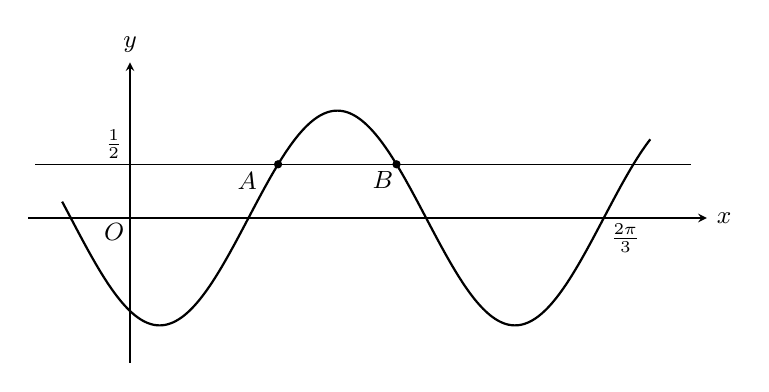
\begin{tikzpicture}
\begin{axis}[width=10.2cm, height=5.4cm, font=\small,
  axis lines=middle, xlabel={$x$}, ylabel={$y$},
  xmin=-0.45, xmax=2.55, ymin=-1.35, ymax=1.45,
  xtick=\empty, ytick=\empty,
  every axis x label/.style={at={(current axis.right of origin)}, anchor=west},
  every axis y label/.style={at={(current axis.above origin)}, anchor=south}]
  \addplot[domain=-0.42:2.48, samples=2] {0.5};
  \addplot[domain=-0.30:2.30, samples=300, thick] {sin(deg(4*x-2*pi/3))};
  \fill (axis cs:0.65450,0.5) circle (1.5pt);
  \fill (axis cs:1.17810,0.5) circle (1.5pt);
  \node[anchor=south east, inner sep=1pt] at (axis cs:-0.02,0.52) {$\frac{1}{2}$};
  \node[anchor=north east, inner sep=1pt] at (axis cs:0.575,0.455) {$A$};
  \node[anchor=north east, inner sep=1pt] at (axis cs:1.178,0.46) {$B$};
  \node[anchor=north west, inner sep=1pt] at (axis cs:2.11,-0.02) {$\frac{2\pi}{3}$};
  \node[anchor=north east, inner sep=1pt] at (axis cs:-0.01,-0.02) {$O$};
\end{axis}
\end{tikzpicture}
\end{center}

\textbf{解析}

\textbf{第一步，从图上读出 $A$、$B$ 的位置关系（这是本题的信息来源）。}

图中 $A$、$B$ 位于\textbf{同一个"波峰"的两侧}：$A$ 在上升段与 $y=\dfrac12$ 相交，$B$ 在下降段相交，二者之间夹着一个最大值点。由于 $A$、$B$ 都在水平线 $y=\dfrac12$ 上，$|AB|$ 就是它们的\textbf{横坐标之差}。

\textbf{第二步，由 $|AB|$ 定 $\omega$。}

在一个周期内解 $\sin\theta=\dfrac12$（其中 $\theta=\omega x+\varphi$）：
\[\theta_A=\frac\pi6\ (\text{\text{上升}}),\qquad \theta_B=\frac{5\pi}6\ (\text{\text{下降}})\]

于是
\[\omega\left(x_B-x_A\right)=\theta_B-\theta_A=\frac{5\pi}6-\frac\pi6=\frac{2\pi}3\]

代入 $x_B-x_A=|AB|=\dfrac\pi6$：
\[\omega\cdot\frac\pi6=\frac{2\pi}3\ \Longrightarrow\ \omega=4\]

\textbf{第三步，由图上标注的零点定 $\varphi$。}

图中标出 $x=\dfrac{2\pi}3$ 处曲线\textbf{由下向上穿过 $x$ 轴}（上升零点），故
\[4\cdot\frac{2\pi}3+\varphi=2k\pi\ (k\in\mathbf Z)\ \Longrightarrow\ \varphi=2k\pi-\frac{8\pi}3\]

取 $k=1$ 得 $\varphi=2\pi-\dfrac{8\pi}3=-\dfrac{2\pi}3$（满足 $|\varphi|<\pi$）。

\textbf{第四步，求 $f(\pi)$。}
\[f(\pi)=\sin\left(4\pi-\frac{2\pi}3\right)=\sin\left(-\frac{2\pi}3\right)=-\frac{\sqrt3}2\]

\textbf{为什么不受 $k$ 的选取影响}：$f(\pi)=\sin(4\pi+\varphi)=\sin\varphi$，而不同的 $k$ 只让 $\varphi$ 相差 $2\pi$ 的整数倍，$\sin\varphi$ 不变。

\textbf{图形一致性核验}（$\omega=4$，$\varphi=-\dfrac{2\pi}3$）：

\begin{center}
\begin{tabular}{ccc}
\toprule
图上特征 & 计算值 & 与图对照 \\
\midrule
$x=0$ 处的函数值 & $\sin\left(-\frac{2\pi}3\right)=-\frac{\sqrt3}2<0$ & 曲线在 $O$ 下方  \\
$O$ 右侧第一个最小值点 & $4x-\frac{2\pi}3=-\frac\pi2\Rightarrow x=\frac\pi{24}\approx0.13$ & 紧邻 $O$ 右侧  \\
$A$、$B$ 的横坐标 & $\approx0.654$、$\approx1.178$ & 差 $\approx0.5236=\frac\pi6$  \\
右端上升零点 & $x=\frac{2\pi}3\approx2.094$ & 与标注一致  \\
\bottomrule
\end{tabular}
\end{center}

\gkanswer{答案：$-\dfrac{\sqrt3}2$}

\begin{gktip}
\textbf{读图要点}：$|AB|$ 是\textbf{两交点间的水平距离}而非弧长；$A$、$B$ 是否在同一波峰两侧决定了 $\theta$ 之差取 $\dfrac{2\pi}3$ 还是 $2\pi-\dfrac{2\pi}3=\dfrac{4\pi}3$（后者对应"跨一个波谷"的相邻交点），\textbf{看错会把 $\omega$ 算成 $8$}。

\textbf{另一个常用关系}：若 $A$、$B$ 在同一波峰两侧，则波峰的横坐标恰是 $\dfrac{x_A+x_B}2$——本题也可先由此定出最大值点再求 $\varphi$。
\end{gktip}

\par\medskip

\gkpart{四、解答题（共 70 分）}

\gksolhead{17}{10 分}

\textbf{题目}　记 $\triangle ABC$ 的内角 $A$，$B$，$C$ 的对边分别为 $a$，$b$，$c$，已知 $\triangle ABC$ 面积为 $\sqrt3$，$D$ 为 $BC$ 的中点，且 $AD=1$。(1) 若 $\angle ADC=\dfrac\pi3$，求 $\tan B$；(2) 若 $b^{2}+c^{2}=8$，求 $b$，$c$。

\par\medskip

\textbf{(1) 解}

\textbf{第一步，用面积定出 $BD=DC$。}

因 $D$ 是 $BC$ 的中点，$\triangle ABD$ 与 $\triangle ADC$ \textbf{等底同高、面积相等}：
\[S_{\triangle ABC}=2S_{\triangle ADC}\]

设 $BD=DC=m$，在 $\triangle ADC$ 中以 $AD$、$DC$ 为夹边：
\[S_{\triangle ADC}=\frac12\cdot AD\cdot DC\cdot\sin\angle ADC=\frac12\times1\times m\times\sin\frac\pi3=\frac{\sqrt3}4m\]

于是
\[S_{\triangle ABC}=2\times\frac{\sqrt3}4m=\frac{\sqrt3}2m=\sqrt3\ \Longrightarrow\ m=2\]

即 $BD=DC=2$，$a=BC=4$。

\textbf{第二步，建系求 $\tan B$（比反复用余弦定理更快）。}

以 $D$ 为原点、射线 $DC$ 为 $x$ 轴正方向建系：
\[D(0,0),\qquad C(2,0),\qquad B(-2,0)\]

$\angle ADC=\dfrac\pi3$ 且 $AD=1$，故 $A$ 在与 $x$ 轴正向成 $60^\circ$ 的方向上：
\[A\left(\cos\frac\pi3,\ \sin\frac\pi3\right)=\left(\frac12,\ \frac{\sqrt3}2\right)\]

角 $B$ 是射线 $BA$ 与射线 $BC$（即 $x$ 轴正向）的夹角，故 $\tan B$ 就是 $BA$ 的斜率：
\[\tan B=\frac{\dfrac{\sqrt3}2-0}{\dfrac12-(-2)}=\frac{\dfrac{\sqrt3}2}{\dfrac52}=\frac{\sqrt3}5\]

\textbf{第三步，用余弦定理独立复核。}

在 $\triangle ABD$ 中，$\angle ADB=\pi-\dfrac\pi3=\dfrac{2\pi}3$：
\[AB^{2}=AD^{2}+BD^{2}-2\cdot AD\cdot BD\cos\frac{2\pi}3=1+4-2\times1\times2\times\left(-\frac12\right)=7\]

\[c=AB=\sqrt7\]

再在 $\triangle ABD$ 中对角 $B$ 用余弦定理：
\[\cos B=\frac{AB^{2}+BD^{2}-AD^{2}}{2\cdot AB\cdot BD}=\frac{7+4-1}{2\sqrt7\times2}=\frac{10}{4\sqrt7}=\frac5{2\sqrt7}\]

\[\sin B=\sqrt{1-\frac{25}{28}}=\sqrt{\frac3{28}}=\frac{\sqrt3}{2\sqrt7}\ \Longrightarrow\ \tan B=\frac{\sqrt3/\left(2\sqrt7\right)}{5/\left(2\sqrt7\right)}=\frac{\sqrt3}5\]

两法一致。

\textbf{所以 $\tan B=\dfrac{\sqrt3}5$。}

\par\medskip

\textbf{(2) 解}

\textbf{第一步，用中线向量公式把 $AD=1$ 翻译成 $bc\cos A$。}

$D$ 为 $BC$ 中点，故
\[\overrightarrow{AD}=\frac12\left(\overrightarrow{AB}+\overrightarrow{AC}\right)\]

两边平方（注意 $\left|\overrightarrow{AB}\right|=c$、$\left|\overrightarrow{AC}\right|=b$、$\overrightarrow{AB}\cdot\overrightarrow{AC}=bc\cos A$）：
\[AD^{2}=\frac14\left(c^{2}+b^{2}+2bc\cos A\right)\]

代入 $AD=1$、$b^{2}+c^{2}=8$：
\[1=\frac14\left(8+2bc\cos A\right)\ \Longrightarrow\ 4=8+2bc\cos A\ \Longrightarrow\ bc\cos A=-2\tag{$*$}\]

\textbf{第二步，用面积得到 $bc\sin A$。}
\[S=\frac12bc\sin A=\sqrt3\ \Longrightarrow\ bc\sin A=2\sqrt3\tag{$**$}\]

\textbf{第三步，两式相除定角、平方相加定 $bc$。}

$(\ast\ast)\div(\ast)$：
\[\tan A=\frac{2\sqrt3}{-2}=-\sqrt3\]

$A\in(0,\pi)$，故
\[A=\frac{2\pi}3\]

$(\ast)^{2}+(\ast\ast)^{2}$（利用 $\sin^{2}A+\cos^{2}A=1$）：
\[(bc)^{2}=(-2)^{2}+\left(2\sqrt3\right)^{2}=4+12=16\ \Longrightarrow\ bc=4\quad(bc>0)\]

\textbf{第四步，由「和」与「积」解出 $b$、$c$。}
\[b^{2}+c^{2}=8,\qquad bc=4\ \Longrightarrow\ (b-c)^{2}=b^{2}+c^{2}-2bc=8-8=0\]

故 $b=c$，再由 $b^{2}+c^{2}=2b^{2}=8$ 得
\[b=c=2\]

\textbf{第五步，回代验证（三个条件全查）。}

\begin{itemize}
\item $b^{2}+c^{2}=4+4=8$ 
\item $a^{2}=b^{2}+c^{2}-2bc\cos A=8-2\times4\times\left(-\dfrac12\right)=12$，$a=2\sqrt3$；中线长
\end{itemize}
\[AD=\frac12\sqrt{2b^{2}+2c^{2}-a^{2}}=\frac12\sqrt{8+8-12}=\frac12\times2=1\ \]
\begin{itemize}
\item $S=\dfrac12bc\sin A=\dfrac12\times4\times\dfrac{\sqrt3}2=\sqrt3$ 
\end{itemize}

\textbf{所以 $b=c=2$。}

\begin{gktip}
\textbf{方法总结}：中线问题有两条主干路径——
1. \textbf{向量法}：$\overrightarrow{AD}=\dfrac12\left(\overrightarrow{AB}+\overrightarrow{AC}\right)$ 平方，一步得到含 $bc\cos A$ 的关系（本题 (2) 用的就是它）；
2. \textbf{中线长公式}：$AD^{2}=\dfrac{2b^{2}+2c^{2}-a^{2}}4$，本质与前者等价，适合直接求边。

而 $(\ast)$ 与 $(\ast\ast)$ 这对「$bc\cos A$ 与 $bc\sin A$ 同时已知」的结构是\textbf{万能配置}：相除得 $\tan A$、平方和得 $bc$，两个未知量一次性解决。第 (1) 问的建系法则展示了另一条思路——\textbf{中点在原点、中线为已知向量}时，坐标法几乎不用算。
\end{gktip}

\par\medskip

\gksolhead{18}{12 分}

\textbf{题目}　已知 $\left\{a_n\right\}$ 为等差数列，$b_n=\begin{cases}a_n-6,&n\ \text{\text{为奇数}}\\ 2a_n,&n\ \text{\text{为偶数}}\end{cases}$，记 $S_n$，$T_n$ 分别为数列 $\left\{a_n\right\}$，$\left\{b_n\right\}$ 的前 $n$ 项和，$S_4=32$，$T_3=16$。(1) 求 $\left\{a_n\right\}$ 的通项公式；(2) 证明：当 $n>5$ 时，$T_n>S_n$。

\par\medskip

\textbf{(1) 解}

设首项 $a_1$、公差 $d$，则 $a_n=a_1+(n-1)d$。

\textbf{第一个方程（由 $S_4=32$）：}
\[S_4=4a_1+\frac{4\times3}2d=4a_1+6d=32\ \Longrightarrow\ 2a_1+3d=16\tag{①}\]

\textbf{第二个方程（由 $T_3=16$）：}

$n=1,3$ 为奇数、$n=2$ 为偶数：
\[T_3=b_1+b_2+b_3=\left(a_1-6\right)+2a_2+\left(a_3-6\right)\]

\[=\left(a_1+a_3\right)+2a_2-12=2a_2+2a_2-12=4a_2-12\]

（这里用了等差数列的性质 $a_1+a_3=2a_2$，可省一步展开。）
\[4a_2-12=16\ \Longrightarrow\ a_2=7\ \Longrightarrow\ a_1+d=7\tag{②}\]

\textbf{解方程组：} 由 ② 得 $a_1=7-d$，代入 ①：
\[2(7-d)+3d=16\ \Longrightarrow\ 14+d=16\ \Longrightarrow\ d=2,\qquad a_1=5\]

\[\boxed{a_n=5+2(n-1)=2n+3}\]

\textbf{验证}：$a_1,a_2,a_3,a_4=5,7,9,11$，$S_4=5+7+9+11=32$ ；
$b_1=5-6=-1$，$b_2=2\times7=14$，$b_3=9-6=3$，$T_3=-1+14+3=16$ 

\par\medskip

\textbf{(2) 证明要点}

\textbf{思路}：不直接算 $T_n$，而是\textbf{逐项作差}——$b_n$ 与 $a_n$ 的关系按奇偶只有两种，差值结构非常简单。

\textbf{第一步，写出 $S_n$ 与逐项差。}
\[S_n=\frac{n\left(a_1+a_n\right)}2=\frac{n(5+2n+3)}2=n(n+4)=n^{2}+4n\]

\[b_n-a_n=\begin{cases}-6,&n\ \text{\text{为奇数}}\\ a_n,&n\ \text{\text{为偶数}}\end{cases}\]

于是
\[T_n-S_n=\sum_{k=1}^{n}\left(b_k-a_k\right)=-6\times\left(1\sim n\ \text{\text{中奇数的个数}}\right)+\sum_{\substack{k\le n\\ k\ \text{\text{为偶数}}}}a_k\]

\textbf{第二步，算偶数项之和。} 偶数下标写成 $k=2j$：
\[a_{2j}=2(2j)+3=4j+3\]

若 $1\sim n$ 中偶数下标为 $2,4,\dots,2m$（共 $m$ 项）：
\[\sum_{j=1}^{m}(4j+3)=4\cdot\frac{m(m+1)}2+3m=2m(m+1)+3m=2m^{2}+5m\]

\textbf{第三步，按 $n$ 的奇偶分两种情形。}

\textbf{情形一：$n=2m$（偶数，$m\ge1$）。} 奇数下标 $1,3,\dots,2m-1$ 共 $m$ 个：
\[T_n-S_n=-6m+\left(2m^{2}+5m\right)=2m^{2}-m=m(2m-1)\]

$n>5$ 且为偶数 $\Rightarrow n\ge6\Rightarrow m\ge3$，而 $m(2m-1)$ 在 $m\ge1$ 时递增：
\[T_n-S_n\ge3\times5=15>0\]

\textbf{情形二：$n=2m+1$（奇数，$m\ge0$）。} 奇数下标 $1,3,\dots,2m+1$ 共 $m+1$ 个，偶数下标仍为 $2,\dots,2m$（共 $m$ 个）：
\[T_n-S_n=-6(m+1)+\left(2m^{2}+5m\right)=2m^{2}-m-6=(2m+3)(m-2)\]

$n>5$ 且为奇数 $\Rightarrow n\ge7\Rightarrow m\ge3$：
\[T_n-S_n\ge(2\times3+3)(3-2)=9>0\]

\textbf{第四步，合并结论。}

两种情形下均有 $T_n-S_n>0$，故
\[T_n>S_n\qquad(n>5)\qquad\blacksquare\]

\textbf{边界核验（说明条件 $n>5$ 是紧的）：}

\begin{center}
\begin{tabular}{cccc}
\toprule
$n$ & $S_n$ & $T_n$ & $T_n-S_n$ \\
\midrule
$4$ & $32$ & $38$ & $+6$ \\
$5$ & $45$ & $45$ & $0$ \\
$6$ & $60$ & $75$ & $+15$ \\
$7$ & $77$ & $86$ & $+9$ \\
$8$ & $96$ & $124$ & $+28$ \\
\bottomrule
\end{tabular}
\end{center}

$n=5$ 处\textbf{恰好相等}——这正是题目要求 $n>5$ 而非 $n\ge5$ 的原因。注意 $T_n-S_n$ 并非单调（$n=6$ 时 $15$、$n=7$ 时 $9$），故必须\textbf{分奇偶}讨论，不能只验一个"最小情形"就说"之后更大"。

\begin{gktip}
\textbf{方法总结}：分段定义数列求和，\textbf{永远优先考虑与已知数列逐项作差}——本题若硬算 $T_n$ 要分奇偶各推一次求和公式，作差后每项只剩 $-6$ 或 $a_n$，工作量减半。

\textbf{踩坑提示}：$T_n-S_n$ 在偶数列与奇数列上分别递增，但\textbf{交错排列时整体不单调}。答题时若写"当 $n=6$ 时已大于 $0$，且差值递增，故 $n>5$ 时成立"，会因为 $n=7$ 处差值反而变小而\textbf{逻辑不成立}，必须两条分支各自估界。
\end{gktip}

\par\medskip

\gksolhead{19}{12 分}

\textbf{题目}　某研究小组经过研究发现某种疾病的患病者与未患病者的某项医学指标有明显差异，经过大量调查，得到如下的患病者和未患病者该指标的频率分布直方图：利用该指标制定一个检测标准，需要确定临界值 $c$，将该指标大于 $c$ 的人判定为阳性，小于或等于 $c$ 的人判定为阴性。此检测标准的漏诊率是将患病者判定为阴性的概率，记为 $p(c)$；误诊率是将未患病者判定为阳性的概率，记为 $q(c)$。假设数据在组内均匀分布。以事件发生的频率作为相应事件发生的概率。(1) 当漏诊率 $p(c)=0.5\%$ 时，求临界值 $c$ 和误诊率 $q(c)$；(2) 设函数 $f(c)=p(c)+q(c)$。当 $c\in[95,105]$，求 $f(c)$ 的解析式，并求 $f(c)$ 在区间 $[95,105]$ 的最小值。

\begin{center}% 2023 新高考Ⅱ卷 19：患病者、未患病者两组指标的频率分布直方图（左右并排）
% 绘制依据：源 PDF 原图。组距均为 5，纵轴「频率/组距」，横轴末端标「指标」。
% 左（患病者）刻度 0,95,100,…,130，七组高度 0.002/0.012/0.034/0.036/0.040/0.040/0.036；
% 右（未患病者）刻度 0,70,75,…,105，七组高度 0.038/0.040/0.040/0.036/0.034/0.010/0.002。
% （两组 Σ高度×5 均为 1。）横轴 0 与首刻度之间、纵轴 0 与最低标注之间均画断轴锯齿；
% 每个纵轴标注值处引水平虚线至对应柱顶。
% 版式：纵轴按 h(v)=0.45+(v−0.002)×125 (cm) 线性映射（故 0.002 的间隔恒为 0.25 cm），
% 柱宽 0.52 cm，右图 xshift=5.9 cm，整图宽约 11.9 cm；密集刻度用 \tiny 以免叠字。
\begin{tikzpicture}[font=\small]
  % ================= 左：患病者 =================
  \begin{scope}
    % 断轴的横轴与纵轴
    \draw (0,0) -- (0.10,0);
    \draw (0.10,0) -- (0.16,0.10) -- (0.24,-0.10) -- (0.30,0);
    \draw[->] (0.30,0) -- (4.55,0);
    \draw (0,0) -- (0,0.10);
    \draw (0,0.10) -- (0.09,0.16) -- (-0.09,0.29) -- (0,0.35);
    \draw[->] (0,0.35) -- (0,5.75);
    \node[anchor=north east, inner sep=1.5pt, font=\tiny] at (0,0) {0};
    \node[anchor=north, inner sep=2pt] at (4.85,0) {指标};
    \node[anchor=south, inner sep=3pt]
      at (0,5.75) {$\displaystyle\frac{\mbox{频率}}{\mbox{组距}}$};
    % 纵轴标注 + 水平虚线引至对应柱顶
    \foreach \h/\lab/\xe in {0.45/0.002/0.45, 1.70/0.012/0.97, 4.45/0.034/1.49,
                             4.70/0.036/2.01, 5.20/0.040/2.53} {
      \draw[dashed] (0,\h) -- (\xe,\h);
      \node[anchor=east, inner sep=2pt, font=\tiny] at (0,\h) {\lab};
    }
    % 七个矩形
    \foreach \i/\h in {0/0.45, 1/1.70, 2/4.45, 3/4.70, 4/5.20, 5/5.20, 6/4.70}
      \draw ({0.45+\i*0.52},0) rectangle ({0.45+(\i+1)*0.52},\h);
    % 横轴刻度
    \foreach \i/\lab in {0/95, 1/100, 2/105, 3/110, 4/115, 5/120, 6/125, 7/130} {
      \draw ({0.45+\i*0.52},0) -- ({0.45+\i*0.52},-0.07);
      \node[anchor=north, inner sep=1.5pt, font=\tiny] at ({0.45+\i*0.52},-0.07) {\lab};
    }
    \node at (2.27,-0.95) {患病者};
  \end{scope}
  % ================= 右：未患病者 =================
  \begin{scope}[xshift=5.9cm]
    \draw (0,0) -- (0.10,0);
    \draw (0.10,0) -- (0.16,0.10) -- (0.24,-0.10) -- (0.30,0);
    \draw[->] (0.30,0) -- (4.55,0);
    \draw (0,0) -- (0,0.10);
    \draw (0,0.10) -- (0.09,0.16) -- (-0.09,0.29) -- (0,0.35);
    \draw[->] (0,0.35) -- (0,5.75);
    \node[anchor=north east, inner sep=1.5pt, font=\tiny] at (0,0) {0};
    \node[anchor=north, inner sep=2pt] at (4.85,0) {指标};
    \node[anchor=south, inner sep=3pt]
      at (0,5.75) {$\displaystyle\frac{\mbox{频率}}{\mbox{组距}}$};
    \foreach \h/\lab/\xe in {0.45/0.002/3.57, 1.45/0.010/3.05, 4.45/0.034/2.53,
                             4.70/0.036/2.01, 4.95/0.038/0.45, 5.20/0.040/0.97} {
      \draw[dashed] (0,\h) -- (\xe,\h);
      \node[anchor=east, inner sep=2pt, font=\tiny] at (0,\h) {\lab};
    }
    \foreach \i/\h in {0/4.95, 1/5.20, 2/5.20, 3/4.70, 4/4.45, 5/1.45, 6/0.45}
      \draw ({0.45+\i*0.52},0) rectangle ({0.45+(\i+1)*0.52},\h);
    \foreach \i/\lab in {0/70, 1/75, 2/80, 3/85, 4/90, 5/95, 6/100, 7/105} {
      \draw ({0.45+\i*0.52},0) -- ({0.45+\i*0.52},-0.07);
      \node[anchor=north, inner sep=1.5pt, font=\tiny] at ({0.45+\i*0.52},-0.07) {\lab};
    }
    \node at (2.27,-0.95) {未患病者};
  \end{scope}
\end{tikzpicture}
\end{center}

\par\medskip

\textbf{读图：把两张直方图的数据先抄成表（这一步做扎实，后面全是算术）}

\textbf{患病者}（组距均为 $5$）：

\begin{center}
\begingroup\setlength{\tabcolsep}{4pt}
\begin{tabular}{cccccccc}
\toprule
区间 & $[95,100)$ & $[100,105)$ & $[105,110)$ & $[110,115)$ & $[115,120)$ & $[120,125)$ & $[125,130)$ \\
\midrule
频率/组距 & $0.002$ & $0.012$ & $0.034$ & $0.036$ & $0.040$ & $0.040$ & $0.036$ \\
频率 & $0.01$ & $0.06$ & $0.17$ & $0.18$ & $0.20$ & $0.20$ & $0.18$ \\
\bottomrule
\end{tabular}
\endgroup
\end{center}

\textbf{未患病者}（组距均为 $5$）：

\begin{center}
\begingroup\setlength{\tabcolsep}{4pt}
\begin{tabular}{cccccccc}
\toprule
区间 & $[70,75)$ & $[75,80)$ & $[80,85)$ & $[85,90)$ & $[90,95)$ & $[95,100)$ & $[100,105)$ \\
\midrule
频率/组距 & $0.038$ & $0.040$ & $0.040$ & $0.036$ & $0.034$ & $0.010$ & $0.002$ \\
频率 & $0.19$ & $0.20$ & $0.20$ & $0.18$ & $0.17$ & $0.05$ & $0.01$ \\
\bottomrule
\end{tabular}
\endgroup
\end{center}

\textbf{读图自检（必做）}：所有小矩形面积之和应为 $1$。
\begin{itemize}
\item 患病者：$(0.002+0.012+0.034+0.036+0.040+0.040+0.036)\times5=0.200\times5=1$ 
\item 未患病者：$(0.038+0.040+0.040+0.036+0.034+0.010+0.002)\times5=0.200\times5=1$ 
\end{itemize}

\par\medskip

\textbf{(1) 解}

\textbf{第一步，写出 $p(c)$ 在 $[95,100]$ 上的表达式。}

$p(c)=P(\text{\text{患病者指标}}\le c)$。患病者指标从 $95$ 开始，第一组 $[95,100)$ 的频率/组距为 $0.002$，组内均匀分布，故当 $95\le c\le100$ 时
\[p(c)=0.002\times(c-95)\]

\textbf{第二步，解出 $c$。}
\[0.002(c-95)=0.005\ \Longrightarrow\ c-95=2.5\ \Longrightarrow\ c=97.5\]

（$97.5$ 确在 $[95,100]$ 内，所用表达式有效 ）

\textbf{第三步，算误诊率 $q(97.5)$。}

$q(c)=P(\text{\text{未患病者指标}}>c)$。$c=97.5$ 落在未患病者的 $[95,100)$ 组内，故
\[q(97.5)=\underbrace{0.010\times(100-97.5)}_{[97.5,\,100)\ \text{\text{部分}}}+\underbrace{0.002\times5}_{[100,\,105)\ \text{\text{整组}}}=0.025+0.010=0.035\]

\textbf{所以临界值 $c=97.5$，误诊率 $q(c)=0.035=3.5\%$。}

\par\medskip

\textbf{(2) 解}

因为 $c=100$ 是两条分布的分段点（患病者由 $[95,100)$ 进入 $[100,105)$，未患病者由 $[95,100)$ 进入 $[100,105)$），需在 $[95,100]$ 与 $[100,105]$ 上分别推导。

\textbf{情形一：$95\le c<100$。}
\[p(c)=0.002(c-95)=0.002c-0.19\]
\[q(c)=\underbrace{0.010\times(100-c)}_{(c,\,100)}+\underbrace{0.002\times5}_{[100,\,105)}=1-0.01c+0.01=1.01-0.01c\]
\[f(c)=p(c)+q(c)=(0.002c-0.19)+(1.01-0.01c)=-0.008c+0.82\]

\textbf{情形二：$100\le c\le105$。}
\[p(c)=\underbrace{0.002\times5}_{[95,\,100)\ \text{\text{整组}}}+\underbrace{0.012\times(c-100)}_{[100,\,c]}=0.01+0.012c-1.2=0.012c-1.19\]
\[q(c)=0.002\times(105-c)=0.21-0.002c\]
\[f(c)=(0.012c-1.19)+(0.21-0.002c)=0.01c-0.98\]

\textbf{解析式：}
\[f(c)=\begin{cases}-0.008c+0.82,&95\le c<100\\ 0.01c-0.98,&100\le c\le105\end{cases}\]

\textbf{第三步，求最小值。}

\begin{itemize}
\item 在 $[95,100)$ 上 $f$ 是斜率 $-0.008<0$ 的一次函数，\textbf{单调递减}，右端趋于 $f(100^{-})=-0.8+0.82=0.02$；
\item 在 $[100,105]$ 上 $f$ 是斜率 $0.01>0$ 的一次函数，\textbf{单调递增}，左端 $f(100)=1-0.98=0.02$。
\end{itemize}

两段在 $c=100$ 处\textbf{衔接连续}（都等于 $0.02$），且 $f$ 呈"先减后增"的 V 形，故
\[f(c)_{\min}=f(100)=0.02\]

\textbf{端点核验}：$f(95)=-0.76+0.82=0.06$（即 $p=0$、$q=0.06$ ）；$f(105)=1.05-0.98=0.07$（即 $p=0.07$、$q=0$ ）。两端都大于 $0.02$，与 V 形一致。

\textbf{所以 $f(c)$ 的解析式如上，在 $[95,105]$ 上的最小值为 $f(100)=0.02$。}

\begin{gktip}
\textbf{实际意义}：$f(c)=p(c)+q(c)$ 是「漏诊 $+$ 误诊」的总错误率。$c$ 定得太低会把大量健康人误判为阳性（$q$ 大），定得太高会漏掉大量患者（$p$ 大），最优临界值 $c=100$ 恰好落在两条分布的\textbf{交叠区边界}上——这正是医学检验中 ROC 曲线选阈值的朴素版本。

\textbf{计算要诀}：「组内均匀分布」意味着\textbf{频率按长度成比例切分}，落在某组内部的 $c$ 只需按比例取该组面积的一部分，其余整组直接乘 $5$。列表后逐段累加，比硬记公式稳妥。
\end{gktip}

\par\medskip

\gksolhead{20}{12 分}

\textbf{题目}　如图，三棱锥 $A\text{-}BCD$ 中，$DA=DB=DC$，$BD\perp CD$，$\angle ADB=\angle ADC=60^\circ$，$E$ 为 $BC$ 的中点。(1) 证明：$BC\perp DA$；(2) 点 $F$ 满足 $\overrightarrow{EF}=\overrightarrow{DA}$，求二面角 $D\text{-}AB\text{-}F$ 的正弦值。

\begin{center}% 2023 新高考Ⅱ卷 20：三棱锥 A-BCD（E 为 BC 中点，点 F 满足 EF→=DA→）
% 绘制依据：源 PDF 原图 + 题设坐标 D(0,0,0)、B(2,0,0)、C(0,2,0)、A(1,1,√2)、
% E(1,1,0)（BC 中点）、F(2,2,√2)。投影：画布 = x·(1,0) + y·(0.42,0.30) + z·(0,1)，
% 得 D(0,0)、B(2,0)、C(0.84,0.60)、E(1.42,0.30)、A(1.42,1.714)、F(2.84,2.014)，
% 版面即 D 左下、B 右下（DB 近水平）、C 中部偏左（被遮挡顶点）、E 中央偏下、
% A 上方中偏左、F 右上角。实线 DB、DA、AB、AF、FB；虚线 DC、CB、CA 及 AE、DE。
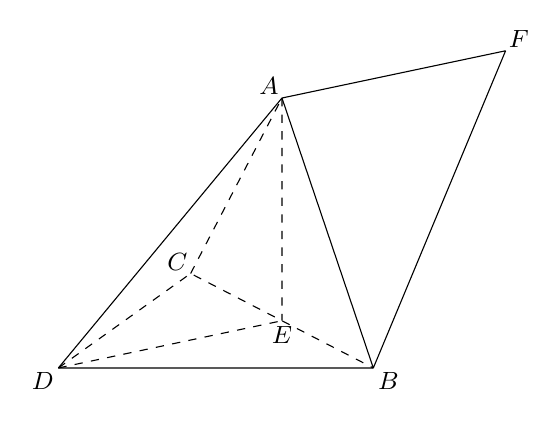
\begin{tikzpicture}[scale=2.0, font=\small]
  \coordinate (D) at (0,0);
  \coordinate (B) at (2,0);
  \coordinate (C) at (0.84,0.60);
  \coordinate (E) at (1.42,0.30);
  \coordinate (A) at (1.42,1.7142);
  \coordinate (F) at (2.84,2.0142);
  \draw (D) -- (B)  (D) -- (A)  (A) -- (B)  (A) -- (F)  (F) -- (B);
  \draw[dashed] (D) -- (C) -- (B);
  \draw[dashed] (C) -- (A);
  \draw[dashed] (A) -- (E)  (D) -- (E);
  \node[below left, inner sep=1.5pt] at (D) {$D$};
  \node[below right, inner sep=1.5pt] at (B) {$B$};
  \node[above left, inner sep=1pt] at (C) {$C$};
  \node[below, inner sep=2pt] at (E) {$E$};
  \node[above left, inner sep=1pt] at (A) {$A$};
  \node[above right, inner sep=1pt] at (F) {$F$};
\end{tikzpicture}
\end{center}

\par\medskip

\textbf{(1) 证明要点}

\textbf{思路}：证「线 $\perp$ 线」的标准路线是先证「线 $\perp$ 面」。目标是把 $DA$ 塞进某个与 $BC$ 垂直的平面。

\textbf{第一步，证 $AB=AC$。}

在 $\triangle ABD$ 与 $\triangle ACD$ 中：
\[DA=DA\ (\text{\text{公共边}}),\qquad \angle ADB=\angle ADC=60^\circ,\qquad DB=DC\]

由 \textbf{SAS} 得 $\triangle ABD\cong\triangle ACD$，故
\[AB=AC\]

\textbf{第二步，用两个等腰三角形的中线。}

$E$ 是 $BC$ 的中点：

\begin{itemize}
\item $\triangle ABC$ 中 $AB=AC$，故中线 $AE\perp BC$；
\item $\triangle DBC$ 中 $DB=DC$，故中线 $DE\perp BC$。
\end{itemize}

\textbf{第三步，线面垂直判定。}

$AE\subset$ 平面 $ADE$，$DE\subset$ 平面 $ADE$，且 $AE\cap DE=E$，故
\[BC\perp\text{\text{平面}}\ ADE\]

而 $DA\subset$ 平面 $ADE$，由线面垂直的性质得
\[BC\perp DA\qquad\blacksquare\]

\begin{gktip}
\textbf{补充}：由 $DA=DB$ 且 $\angle ADB=60^\circ$ 知 $\triangle ABD$ 是\textbf{等边三角形}，故 $AB=DA$；同理 $AC=DA$。这个结论在第 (2) 问建系后可用来验算。
\end{gktip}

\par\medskip

\textbf{(2) 解}

\textbf{第一步，建立空间直角坐标系。}

题设中 $BD\perp CD$，这提供了现成的两条互相垂直的棱。不妨设
\[DA=DB=DC=2\]
（二面角只与形状有关、与整体缩放无关，取 $2$ 可避免分数。）

以 $D$ 为原点、$\overrightarrow{DB}$ 方向为 $x$ 轴、$\overrightarrow{DC}$ 方向为 $y$ 轴、垂直于平面 $BDC$ 向上为 $z$ 轴：
\[D(0,0,0),\qquad B(2,0,0),\qquad C(0,2,0)\]

\textbf{第二步，定出 $A$ 的坐标。}

设 $A(x,y,z)$，$z>0$。由 $\angle ADB=60^\circ$：
\[\cos60^\circ=\frac{\overrightarrow{DA}\cdot\overrightarrow{DB}}{\left|\overrightarrow{DA}\right|\left|\overrightarrow{DB}\right|}=\frac{2x}{2\times2}=\frac x2=\frac12\ \Longrightarrow\ x=1\]

同理由 $\angle ADC=60^\circ$ 得 $y=1$。再由 $\left|\overrightarrow{DA}\right|=2$：
\[1^{2}+1^{2}+z^{2}=4\ \Longrightarrow\ z=\sqrt2\]

\[A\left(1,1,\sqrt2\right)\]

\textbf{核验}：$AB=\left|\left(1,-1,-\sqrt2\right)\right|=\sqrt{1+1+2}=2=DA$ （与 (1) 中「$\triangle ABD$ 等边」一致）；
$\overrightarrow{BC}\cdot\overrightarrow{DA}=(-2,2,0)\cdot\left(1,1,\sqrt2\right)=-2+2+0=0$ （第 (1) 问的坐标验证）。

\textbf{第三步，定出 $E$ 与 $F$。}
\[E=\frac{B+C}2=(1,1,0)\]

由 $\overrightarrow{EF}=\overrightarrow{DA}=\left(1,1,\sqrt2\right)$：
\[F=E+\left(1,1,\sqrt2\right)=\left(2,2,\sqrt2\right)\]

\textbf{第四步，求两个半平面所在平面的法向量。}

\textbf{平面 $ABD$}（含 $D$、$A$、$B$）：取
\[\boldsymbol n_1=\overrightarrow{DA}\times\overrightarrow{DB}=\left(1,1,\sqrt2\right)\times(2,0,0)\]
\[=\left(1\times0-\sqrt2\times0,\ \ \sqrt2\times2-1\times0,\ \ 1\times0-1\times2\right)=\left(0,\ 2\sqrt2,\ -2\right)\]

\textbf{平面 $ABF$}（含 $A$、$B$、$F$）：
\[\overrightarrow{AB}=B-A=\left(1,-1,-\sqrt2\right),\qquad \overrightarrow{AF}=F-A=(1,1,0)\]
\[\boldsymbol n_2=\overrightarrow{AB}\times\overrightarrow{AF}=\left((-1)\times0-\left(-\sqrt2\right)\times1,\ \ \left(-\sqrt2\right)\times1-1\times0,\ \ 1\times1-(-1)\times1\right)\]
\[=\left(\sqrt2,\ -\sqrt2,\ 2\right)\]

\textbf{第五步，求夹角。}
\[\boldsymbol n_1\cdot\boldsymbol n_2=0\times\sqrt2+2\sqrt2\times\left(-\sqrt2\right)+(-2)\times2=0-4-4=-8\]
\[\left|\boldsymbol n_1\right|=\sqrt{0+8+4}=\sqrt{12}=2\sqrt3,\qquad \left|\boldsymbol n_2\right|=\sqrt{2+2+4}=\sqrt8=2\sqrt2\]
\[\cos\left\langle\boldsymbol n_1,\boldsymbol n_2\right\rangle=\frac{-8}{2\sqrt3\times2\sqrt2}=\frac{-8}{4\sqrt6}=-\frac2{\sqrt6}=-\frac{\sqrt6}3\]

设二面角 $D\text{-}AB\text{-}F$ 为 $\theta$，则 $|\cos\theta|=\dfrac{\sqrt6}3$，于是
\[\sin\theta=\sqrt{1-\cos^{2}\theta}=\sqrt{1-\frac69}=\sqrt{\frac39}=\frac{\sqrt3}3\]

\textbf{所以二面角 $D\text{-}AB\text{-}F$ 的正弦值为 $\dfrac{\sqrt3}3$。}

\begin{gktip}
\textbf{为什么求正弦时不必判断二面角的钝锐}：法向量夹角与二面角要么相等、要么互补，两者的\textbf{正弦值恒相同}（$\sin(\pi-\theta)=\sin\theta$）。题目问正弦值正是为了免去定向讨论——若问余弦值，就必须借助图形或第三点判断二面角是钝角还是锐角了。（本题 $\cos\left\langle\boldsymbol n_1,\boldsymbol n_2\right\rangle<0$ 而 $F$ 在 $E$ 的外侧，实际二面角为钝角，$\cos\theta=-\dfrac{\sqrt6}3$。）

\textbf{建系的选点逻辑}：$BD\perp CD$ 是题设\textbf{唯一现成的直角}，因此把 $D$ 设为原点、$DB$ 与 $DC$ 设为两条坐标轴是最省力的；两个 $60^\circ$ 角随即把 $A$ 的前两个坐标一次性定死，第三个坐标由模长补齐——这是「已知一点到三条轴的夹角」型建系的通法。
\end{gktip}

\par\medskip

\gksolhead{21}{12 分}

\textbf{题目}　已知双曲线 $C$ 的中心为坐标原点，左焦点为 $\left(-2\sqrt5,0\right)$，离心率为 $\sqrt5$。(1) 求 $C$ 的方程；(2) 记 $C$ 的左、右顶点分别为 $A_1$，$A_2$，过点 $(-4,0)$ 的直线与 $C$ 的左支交于 $M$，$N$ 两点，$M$ 在第二象限，直线 $MA_1$ 与直线 $NA_2$ 交于 $P$，证明：点 $P$ 在定直线上。

\par\medskip

\textbf{(1) 解}

左焦点在 $x$ 轴上，故双曲线的焦点在 $x$ 轴上，设
\[C:\frac{x^{2}}{a^{2}}-\frac{y^{2}}{b^{2}}=1\quad(a>0,\ b>0)\]

由左焦点坐标得 $c=2\sqrt5$；由离心率
\[e=\frac ca=\sqrt5\ \Longrightarrow\ a=\frac c{\sqrt5}=\frac{2\sqrt5}{\sqrt5}=2\]

\[a^{2}=4,\qquad b^{2}=c^{2}-a^{2}=20-4=16\]

\[\boxed{C:\ \frac{x^{2}}4-\frac{y^{2}}{16}=1}\]

于是 $A_1(-2,0)$，$A_2(2,0)$。

\par\medskip

\textbf{(2) 证明要点}

\textbf{第一步，设直线并联立。}

直线过 $(-4,0)$ 且与左支交于两点，故它\textbf{不是水平线}（水平线与左支至多一个交点），可设
\[x=my-4\]

代入 $C$ 的方程（先化为 $4x^{2}-y^{2}=16$）：
\[4(my-4)^{2}-y^{2}=16\ \Longrightarrow\ 4m^{2}y^{2}-32my+64-y^{2}=16\]

\[\left(4m^{2}-1\right)y^{2}-32my+48=0\tag{①}\]

由韦达定理
\[y_1+y_2=\frac{32m}{4m^{2}-1},\qquad y_1y_2=\frac{48}{4m^{2}-1}\tag{②}\]

\textbf{参数范围}：$M$、$N$ 都在左支上且分居 $x$ 轴两侧，故 $y_1y_2<0$，由 ② 需 $4m^{2}-1<0$，即
\[-\frac12<m<\frac12\]

（此时 ① 的判别式 $\Delta=(32m)^{2}-4\left(4m^{2}-1\right)\times48=256m^{2}+192>0$ 自动成立。）

\textbf{第二步，把 ② 改写成"积用和表示"的形式——这是本题的枢纽。}

由 ② 两式相除消去 $4m^{2}-1$：
\[\frac{y_1y_2}{y_1+y_2}=\frac{48}{32m}=\frac3{2m}\ \Longrightarrow\ m\,y_1y_2=\frac32\left(y_1+y_2\right)\tag{③}\]

（先处理 $m=0$ 的情形：此时直线为 $x=-4$，由 ① 得 $y^{2}=48$，$M\left(-4,4\sqrt3\right)$、$N\left(-4,-4\sqrt3\right)$，可直接验证，见第四步。以下设 $m\ne0$。）

\textbf{第三步，联立两条直线求交点的横坐标。}

$M\left(x_1,y_1\right)$ 在第二象限（$y_1>0$），$N\left(x_2,y_2\right)$（$y_2<0$）。
\[MA_1:\ y=\frac{y_1}{x_1+2}(x+2),\qquad NA_2:\ y=\frac{y_2}{x_2-2}(x-2)\]

在交点 $P$ 处两式相等，两边相除（$y\ne0$，否则 $P$ 在 $x$ 轴上，与 $M$、$N$ 的位置矛盾）：
\[\frac{x+2}{x-2}=\frac{y_2\left(x_1+2\right)}{y_1\left(x_2-2\right)}\tag{④}\]

代入 $x_i=my_i-4$：
\[x_1+2=my_1-2,\qquad x_2-2=my_2-6\]

\[\frac{y_2\left(my_1-2\right)}{y_1\left(my_2-6\right)}=\frac{m\,y_1y_2-2y_2}{m\,y_1y_2-6y_1}\]

\textbf{用 ③ 把 $m\,y_1y_2$ 全部换成 $\dfrac32\left(y_1+y_2\right)$：}

分子：
\[\frac32\left(y_1+y_2\right)-2y_2=\frac32y_1+\frac32y_2-2y_2=\frac32y_1-\frac12y_2=\frac12\left(3y_1-y_2\right)\]

分母：
\[\frac32\left(y_1+y_2\right)-6y_1=\frac32y_2-\frac92y_1=-\frac32\left(3y_1-y_2\right)\]

\textbf{第四步，说明公因子非零，然后约去。}

若 $3y_1-y_2=0$，则 $y_2=3y_1$，代入 ②：
\[y_1+y_2=4y_1=\frac{32m}{4m^{2}-1},\qquad y_1y_2=3y_1^{2}=\frac{48}{4m^{2}-1}\]

由前式 $y_1=\dfrac{8m}{4m^{2}-1}$，代入后式：
\[3\cdot\frac{64m^{2}}{\left(4m^{2}-1\right)^{2}}=\frac{48}{4m^{2}-1}\ \Longrightarrow\ \frac{192m^{2}}{4m^{2}-1}=48\ \Longrightarrow\ 192m^{2}=192m^{2}-48\]

得 $0=-48$，\textbf{矛盾}。故恒有 $3y_1-y_2\ne0$，可以约去：
\[\frac{y_2\left(x_1+2\right)}{y_1\left(x_2-2\right)}=\frac{\dfrac12\left(3y_1-y_2\right)}{-\dfrac32\left(3y_1-y_2\right)}=-\frac13\]

代回 ④：
\[\frac{x+2}{x-2}=-\frac13\ \Longrightarrow\ 3(x+2)=-(x-2)\ \Longrightarrow\ 3x+6=-x+2\ \Longrightarrow\ x=-1\]

\textbf{第五步，补上 $m=0$ 的情形。}

$M\left(-4,4\sqrt3\right)$，$N\left(-4,-4\sqrt3\right)$：
\[MA_1:\ k=\frac{4\sqrt3-0}{-4-(-2)}=-2\sqrt3,\qquad y=-2\sqrt3(x+2)\]
\[NA_2:\ k=\frac{-4\sqrt3-0}{-4-2}=\frac{2\sqrt3}3,\qquad y=\frac{2\sqrt3}3(x-2)\]

令二者相等：
\[-2\sqrt3(x+2)=\frac{2\sqrt3}3(x-2)\ \Longrightarrow\ -3(x+2)=x-2\ \Longrightarrow\ -4x=4\ \Longrightarrow\ x=-1\ \]

\textbf{结论}：无论直线如何选取，交点 $P$ 的横坐标恒为 $-1$，即
\[P\ \text{\text{在定直线}}\ x=-1\ \text{\text{上}}\qquad\blacksquare\]

\textbf{数值抽验}（独立于上述推导）：

\begin{center}
\begin{tabular}{cccc}
\toprule
$m$ & $M$ & $N$ & $P$ \\
\midrule
$0$ & $\left(-4,\ 6.928\right)$ & $\left(-4,\ -6.928\right)$ & $\left(-1,\ -3.464\right)$ \\
$0.2$ & $\left(-3.069,\ 4.655\right)$ & $\left(-6.455,\ -12.275\right)$ & $\left(-1,\ -4.355\right)$ \\
$-0.3$ & $\left(-9.687,\ 18.956\right)$ & $\left(-2.813,\ -3.956\right)$ & $\left(-1,\ -2.466\right)$ \\
$0.45$ & $\left(-2.561,\ 3.198\right)$ & $\left(-39.54,\ -78.99\right)$ & $\left(-1,\ -5.704\right)$ \\
\bottomrule
\end{tabular}
\end{center}

四组横坐标全为 $-1$ 

\begin{gktip}
\textbf{方法总结——"定点/定直线"题的通用套路}：
1. \textbf{设线用 $x=my+t$ 而非 $y=kx+b$}：过定点且与曲线交于两点的直线常常包含竖直线，用 $x=my+t$ 可一次覆盖（斜率不存在的情形自动含在 $m=0$ 里），只需单独留意 $m=0$ 的化简。
2. \textbf{不解出 $y_1$、$y_2$，只用"和"与"积"}：把韦达定理的两式\textbf{相除}消去参数，得到 ③ 这样的"积用和表示"的桥梁式，代入后目标表达式里的参数会整体消失。
3. \textbf{约分前必须证明公因子非零}——本题 $3y_1-y_2\ne0$ 的验证是完整解答不可省的一环，反证只需两行。

\textbf{为什么答案是 $x=-1$}：$(-4,0)$ 与定直线 $x=-1$ 关于……并非简单对称，而是满足 $x_{\text{\text{定}}}=\dfrac{a^{2}}{x_{\text{\text{过}}}}=\dfrac4{-4}=-1$——这正是双曲线中\textbf{极点与极线}的关系：过点 $(-4,0)$ 的弦的两端点与两顶点连线的交点，恒落在该点关于 $C$ 的极线上。记住这个二级结论可在选择填空题里秒答。
\end{gktip}

\par\medskip

\gksolhead{22}{12 分}

\textbf{题目}　(1) 证明：当 $0<x<1$ 时，$x-x^{2}<\sin x<x$；(2) 已知函数 $f(x)=\cos ax-\ln\left(1-x^{2}\right)$，若 $x=0$ 是 $f(x)$ 的极大值点，求 $a$ 的取值范围。

\par\medskip

\textbf{(1) 证明要点}

\textbf{右半边：$\sin x<x$。}

令
\[u(x)=x-\sin x,\qquad x\in[0,1]\]

\[u'(x)=1-\cos x\ge0\]

且 $u'(x)=0$ 仅在 $x=0$ 处成立（$0<x<1$ 时 $\cos x<1$），故 $u$ 在 $[0,1]$ 上\textbf{严格递增}。由 $u(0)=0$ 得
\[u(x)>0\quad(0<x<1)\ \Longrightarrow\ \sin x<x\]

\textbf{左半边：$x-x^{2}<\sin x$。}

令
\[v(x)=\sin x-x+x^{2},\qquad x\in[0,1]\]

\[v'(x)=\cos x-1+2x,\qquad v''(x)=-\sin x+2\]

因 $|\sin x|\le1$，故 $v''(x)\ge1>0$，$v'$ 在 $[0,1]$ 上\textbf{严格递增}。而
\[v'(0)=\cos0-1+0=0\]

故 $0<x<1$ 时 $v'(x)>0$，$v$ 严格递增。再由 $v(0)=0$ 得
\[v(x)>0\quad(0<x<1)\ \Longrightarrow\ \sin x>x-x^{2}\]

两边合起来即
\[x-x^{2}<\sin x<x\qquad(0<x<1)\qquad\blacksquare\]

\begin{gktip}
\textbf{要点}：右半边一次求导即可；左半边一次求导后 $v'(0)=0$ 无法定号，\textbf{必须再求一次导}把 $v'$ 的单调性弄清楚——这种"二阶求导定一阶符号"的手法在导数压轴题里出现频率极高。
\end{gktip}

\par\medskip

\textbf{(2) 解}

\textbf{第一步，明确定义域与对称性。}

需 $1-x^{2}>0$，故定义域为 $(-1,1)$。又
\[f(-x)=\cos(-ax)-\ln\left(1-x^{2}\right)=\cos ax-\ln\left(1-x^{2}\right)=f(x)\]

故 $f$ 是\textbf{偶函数}；同时 $f$ 只通过 $\cos ax$ 依赖 $a$，而 $\cos(-ax)=\cos ax$，故\textbf{结论关于 $a$ 的符号对称}——只需讨论 $a\ge0$，答案再对称补全。

\textbf{第二步，算出前两阶导数在 $0$ 处的值。}
\[f'(x)=-a\sin ax+\frac{2x}{1-x^{2}}\]
\[f''(x)=-a^{2}\cos ax+\frac{2\left(1+x^{2}\right)}{\left(1-x^{2}\right)^{2}}\]

（第二项求导：$\left(\dfrac{2x}{1-x^{2}}\right)'=\dfrac{2\left(1-x^{2}\right)-2x(-2x)}{\left(1-x^{2}\right)^{2}}=\dfrac{2+2x^{2}}{\left(1-x^{2}\right)^{2}}$。）

代入 $x=0$：
\[f'(0)=0,\qquad f''(0)=2-a^{2}\]

$x=0$ 是\textbf{驻点}（这与 $a$ 无关，由偶函数性质也可直接看出），能否成为极大值点完全取决于 $f''(0)$ 的符号。

\textbf{第三步，分三种情形讨论。}

\textbf{情形一：$a^{2}>2$（即 $|a|>\sqrt2$）——是极大值点 }

$f''(0)=2-a^{2}<0$。因 $f''$ 连续，存在 $\delta>0$ 使 $f''(x)<0$ 在 $(-\delta,\delta)$ 上恒成立，故 $f'$ 在该邻域内\textbf{严格递减}。结合 $f'(0)=0$：
\[x\in(-\delta,0)\Rightarrow f'(x)>0;\qquad x\in(0,\delta)\Rightarrow f'(x)<0\]

即 $f$ 在 $0$ 左侧递增、右侧递减，$x=0$ 是\textbf{极大值点} 

\textbf{情形二：$a^{2}<2$（即 $|a|<\sqrt2$，含 $a=0$）——是极小值点 }

$f''(0)=2-a^{2}>0$，同理 $f''>0$ 在某邻域上成立，$f'$ 严格递增且 $f'(0)=0$，故 $f$ 在 $0$ 左侧递减、右侧递增，$x=0$ 是\textbf{极小值点}，不合题意 

（$a=0$ 时 $f(x)=1-\ln\left(1-x^{2}\right)$，$f'(x)=\dfrac{2x}{1-x^{2}}$，显然在 $0$ 处取极小，可作为特例核验。）

\textbf{情形三：$a^{2}=2$（即 $a=\pm\sqrt2$）——二阶判别失效，需用第 (1) 问 }

此时 $f''(0)=0$。由对称性只需看 $a=\sqrt2$，且由 $f$ 是偶函数只需考察 $0<x<1$。

\[f(x)-f(0)=\cos\left(\sqrt2x\right)-1-\ln\left(1-x^{2}\right)\]

\textbf{估计第一项}（用二倍角公式化成平方，便于用 (1) 的结论）：
\[\cos\left(\sqrt2x\right)-1=-2\sin^{2}\frac{\sqrt2x}2=-2\sin^{2}\frac x{\sqrt2}\]

当 $0<x<1$ 时 $0<\dfrac x{\sqrt2}<1$，由第 (1) 问的\textbf{右半边}：
\[0<\sin\frac x{\sqrt2}<\frac x{\sqrt2}\ \Longrightarrow\ \sin^{2}\frac x{\sqrt2}<\frac{x^{2}}2\ \Longrightarrow\ \cos\left(\sqrt2x\right)-1>-x^{2}\]

\textbf{估计第二项}（用经典不等式 $\ln t\le t-1$，等号仅在 $t=1$ 取到）：取 $t=1-x^{2}<1$：
\[\ln\left(1-x^{2}\right)<\left(1-x^{2}\right)-1=-x^{2}\ \Longrightarrow\ -\ln\left(1-x^{2}\right)>x^{2}\]

\textbf{相加}：
\[f(x)-f(0)>-x^{2}+x^{2}=0\qquad(0<x<1)\]

由 $f$ 为偶函数，$-1<x<0$ 时同样有 $f(x)>f(0)$。故 $x=0$ 是 $f$ 的\textbf{极小值点}（实为最小值点），不合题意 

\textbf{第四步，汇总。}

只有情形一满足「$x=0$ 是极大值点」，即 $|a|>\sqrt2$：
\[\boxed{a\in\left(-\infty,-\sqrt2\right)\cup\left(\sqrt2,+\infty\right)}\]

\textbf{数值抽验}（计算 $f(x)-f(0)$ 在 $x=0.001,\ 0.01,\ 0.03$ 处的符号）：

\begin{center}
\begin{tabular}{ccccc}
\toprule
$a$ & $x=0.001$ & $x=0.01$ & $x=0.03$ & 结论 \\
\midrule
$0$ & $+1.0\times10^{-6}$ & $+1.0\times10^{-4}$ & $+9.0\times10^{-4}$ & 极小  \\
$1.2$ & $+2.8\times10^{-7}$ & $+2.8\times10^{-5}$ & $+2.5\times10^{-4}$ & 极小  \\
$\sqrt2$ & $+6.7\times10^{-13}$ & $+6.7\times10^{-9}$ & $+5.4\times10^{-7}$ & 极小  \\
$1.5$ & $-1.3\times10^{-7}$ & $-1.2\times10^{-5}$ & $-1.1\times10^{-4}$ & 极大  \\
$2$ & $-1.0\times10^{-6}$ & $-1.0\times10^{-4}$ & $-9.0\times10^{-4}$ & 极大  \\
\bottomrule
\end{tabular}
\end{center}

$a=\sqrt2$ 处差值虽然极小（$10^{-13}$ 量级）但\textbf{确为正号}，与情形三的结论一致——这正说明为什么该临界点必须用不等式严格论证，光靠画图或代数值极易误判。

\begin{gktip}
\textbf{方法总结}：
1. \textbf{偶函数 $\Rightarrow f'(0)=0$}：本题 $x=0$ 必是驻点，问题的实质是「驻点的类型」，因此二阶导数的符号是天然突破口。
2. \textbf{$f''(0)=0$ 是分水岭}：$2-a^{2}$ 变号处 $a=\pm\sqrt2$ 必须\textbf{单独处理}，因为二阶判别法在此失效。做题时若只写「$f''(0)<0$ 故 $a^{2}>2$」而不说明 $a^{2}=2$ 为何舍去，会被扣分。
3. \textbf{临界情形的处理靠第 (1) 问}——高考压轴题的两问几乎总是"工具 + 用途"的关系：$\sin x<x$ 恰好把 $\cos\left(\sqrt2x\right)-1$ 压到 $-x^{2}$ 以上，而 $\ln t\le t-1$ 把 $-\ln\left(1-x^{2}\right)$ 顶到 $x^{2}$ 以上，二者\textbf{严丝合缝地抵消}。看到第 (1) 问的形式就该预判它会在第 (2) 问的边界情形登场。

\textbf{展开视角（不必写进答卷，但有助理解）}：在 $x=0$ 附近
\[f(x)=1+\left(1-\frac{a^{2}}2\right)x^{2}+\left(\frac12+\frac{a^{4}}{24}\right)x^{4}+\cdots\]
$x^{2}$ 的系数在 $a^{2}=2$ 时为零，此时由 $x^{4}$ 的系数 $\dfrac12+\dfrac{4}{24}=\dfrac23>0$ 决定，故取极小——与第三种情形的严格证明完全吻合。
\end{gktip}
